\chapter[Microsatellite sequencing permits study of alterations in microsatellite unstable cancers]{Microsatellite sequencing permits study of alterations in microsatellite unstable cancers\footnote{This chapter previously published as: \begin{itemize} \item{Kautto E, Bonneville R, \textit{et al}. Performance evaluation for rapid detection of pan-cancer microsatellite instability with MANTIS\@. \textit{Oncotarget} 2016 [Epub 12 Dec 2016]} \item{Bonneville R\cofirst, Krook MA\cofirst, \textit{et al}. Landscape of microsatellite instability across 39 cancer types. \textit{JCO Precision Oncology} 2017 [Epub 3 Oct 2017]. Reprinted with permission. \textcopyright{} (2017) American Society of Clinical Oncology. All rights reserved.}\end{itemize}}}
\label{ch:msilandscape}

\section{Introduction}
Microsatellites are short (1--6 bp) repeating motifs, widely dispersed throughout the human genome \cite{kelkar2010}. Microsatellite instability (MSI) is a genetic phenomenon of somatic polymorphisms of microsatellite length, caused by uncorrected ``slippage'' of DNA fragments during DNA replication in cell division (Section \ref{ssec:intro:mutation}). MSI can arise from defects in the DNA mismatch repair (MMR) system \cite{shia2015}, which renders cells unable to regulate the lengths of their microsatellites during cell division. These defects may be inherited, as with Lynch syndrome/hereditary nonpolyposis colorectal cancer \cite{lynch1966,aaltonen1993}, or may be somatically acquired, most commonly due to promoter hypermethylation of the MMR gene \textit{MLH1} \cite{armaghany2012}. After multiple cycles of cell division, cells with an impaired MMR system will develop varying lengths in their microsatellite sequences.

Increasing evidence demonstrates that MSI is a recurrent somatic abnormality in several human cancers, previously described in 13\% of colorectal adenocarcinoma and 22-33\% of uterine/endometrial carcinoma \cite{dudley2016}. Reliable detection of MSI is clinically useful as patients with MSI-high (MSI–H) colorectal tumors have been shown to have improved prognosis over those with microsatellite stable (MSS) tumors \cite{buckowitz2005,benatti2005}. Furthermore, MSI-positive tumors appear more susceptible to immune-enhancing therapies, as observed in colorectal cancer for the PD-1 inhibitor pembrolizumab \cite{le2015}, recently approved for any MSI-H or MMR-deficient unresectable or metastatic solid tumor \cite{keytrudafda2017}. Thus far, MSI-H tumors have the highest response rates for any cancer types to PD-1 inhibitors, have durable responses, and a statistically significant improvement in overall survival.

The two currently accepted assays for the detection of MSI are MSI-PCR of five standardized microsatellite loci (Bethesda panel) \cite{boland1998}, and immunohistochemistry (IHC) of the MMR proteins MSH2, MSH6, MLH1 and PMS2. Traditionally, tumors can be classified with MSI-PCR as MSS (0/5 loci unstable), MSI-low (MSI-L, 1/5 loci unstable), or MSI-H ($\ge$2/5 loci unstable). However, both of these methods have inherent limitations. MSI-PCR relies on a small set of loci that were selected based on markers from a single disease type, potentially excluding loci that would be better predictors in other diseases and increasing the odds of incorrect classification \cite{boland1998}. Immunohistochemistry can be used to detect the expression of mismatch repair proteins, but does not directly look at the microsatellite loci. More recently, with the increasing prevalence of next-generation sequencing (NGS) in cancer biology, several computational methods have been developed using either colorectal or endometrial cancer NGS data to determine MSI status \cite{salipante2014,niu2013}.

The development, refinement, and validation of NGS-based computational MSI calling methods have several research and clinical applications. NGS allows for the practical assessment of far more microsatellite loci than MSI-PCR\@. Importantly, computational MSI analyses can be integrated into existing NGS pipelines for other mutation types such as single nucleotide variation or copy number variation, as well as applied to previously generated NGS data for retrospective analyses. As NGS increases in both cost-effectiveness and prevalence, NGS-based methods may permit identification of MSI status without requiring additional clinical testing or patient sample processing. Lastly, NGS data is becoming increasingly available in tumor types that are not routinely tested for MSI, with potential opportunities to identify microsatellite instability in previously uncharacterized cancers. Thus, there is a need to develop tools with high accuracy in multiple cancer types.

In this study, we introduce a new tool, MANTIS (Microsatellite Analysis for Normal Tumor InStability), for detecting MSI status from NGS data. We compare MANTIS with two currently available tools, mSINGS \cite{salipante2014} and MSISensor \cite{niu2013}, and test their performance across six different tumor types. We demonstrate that MANTIS achieves high sensitivity (97\%) and specificity (99\%) across six cancer types. We also determine that the number of loci assessed impacts the accuracy of MSI calling methods, and we find an optimal number of loci to analyze with each tool for best tool performance. As MANTIS performance is most stable with varying numbers of available loci, MANTIS is particularly well suited for application to a wider variety of cancer types.

Clinical MSI testing is routinely performed only on colorectal and endometrial tumors \cite{giardiello2014}, therefore the prevalence of MSI in many other cancer types has been much less well described. Additionally, evidence exists that MSI-PCR may be less accurate in other cancer types \cite{faulkner2004}. A recent study by Hause \textit{et al} \cite{hause2016} developed and applied the MSI detection tool MOSAIC to perform a detailed survey of MSI across 18 cancer types (n=5,930 cases). However, many other cancer types have yet to be analyzed for MSI\@. The ability to detect MSI in novel cancer types would permit investigation of immune-enhancing therapies in these cancers, with the potential to benefit previously unknown subsets of cancer patients with MSI\@.

To perform a more comprehensive assessment of MSI across many additional cancer types than analyzed by Hause \textit{et al}, we applied MANTIS to determine the prevalence of MSI in 39 distinct cancer types (n=11,139 tumors from 11,080 patients).

\section{Materials and Methods}

\subsection{MANTIS}
\label{ssec:msilandscape:mantis}
\begin{figure}[htp]
	\centering
	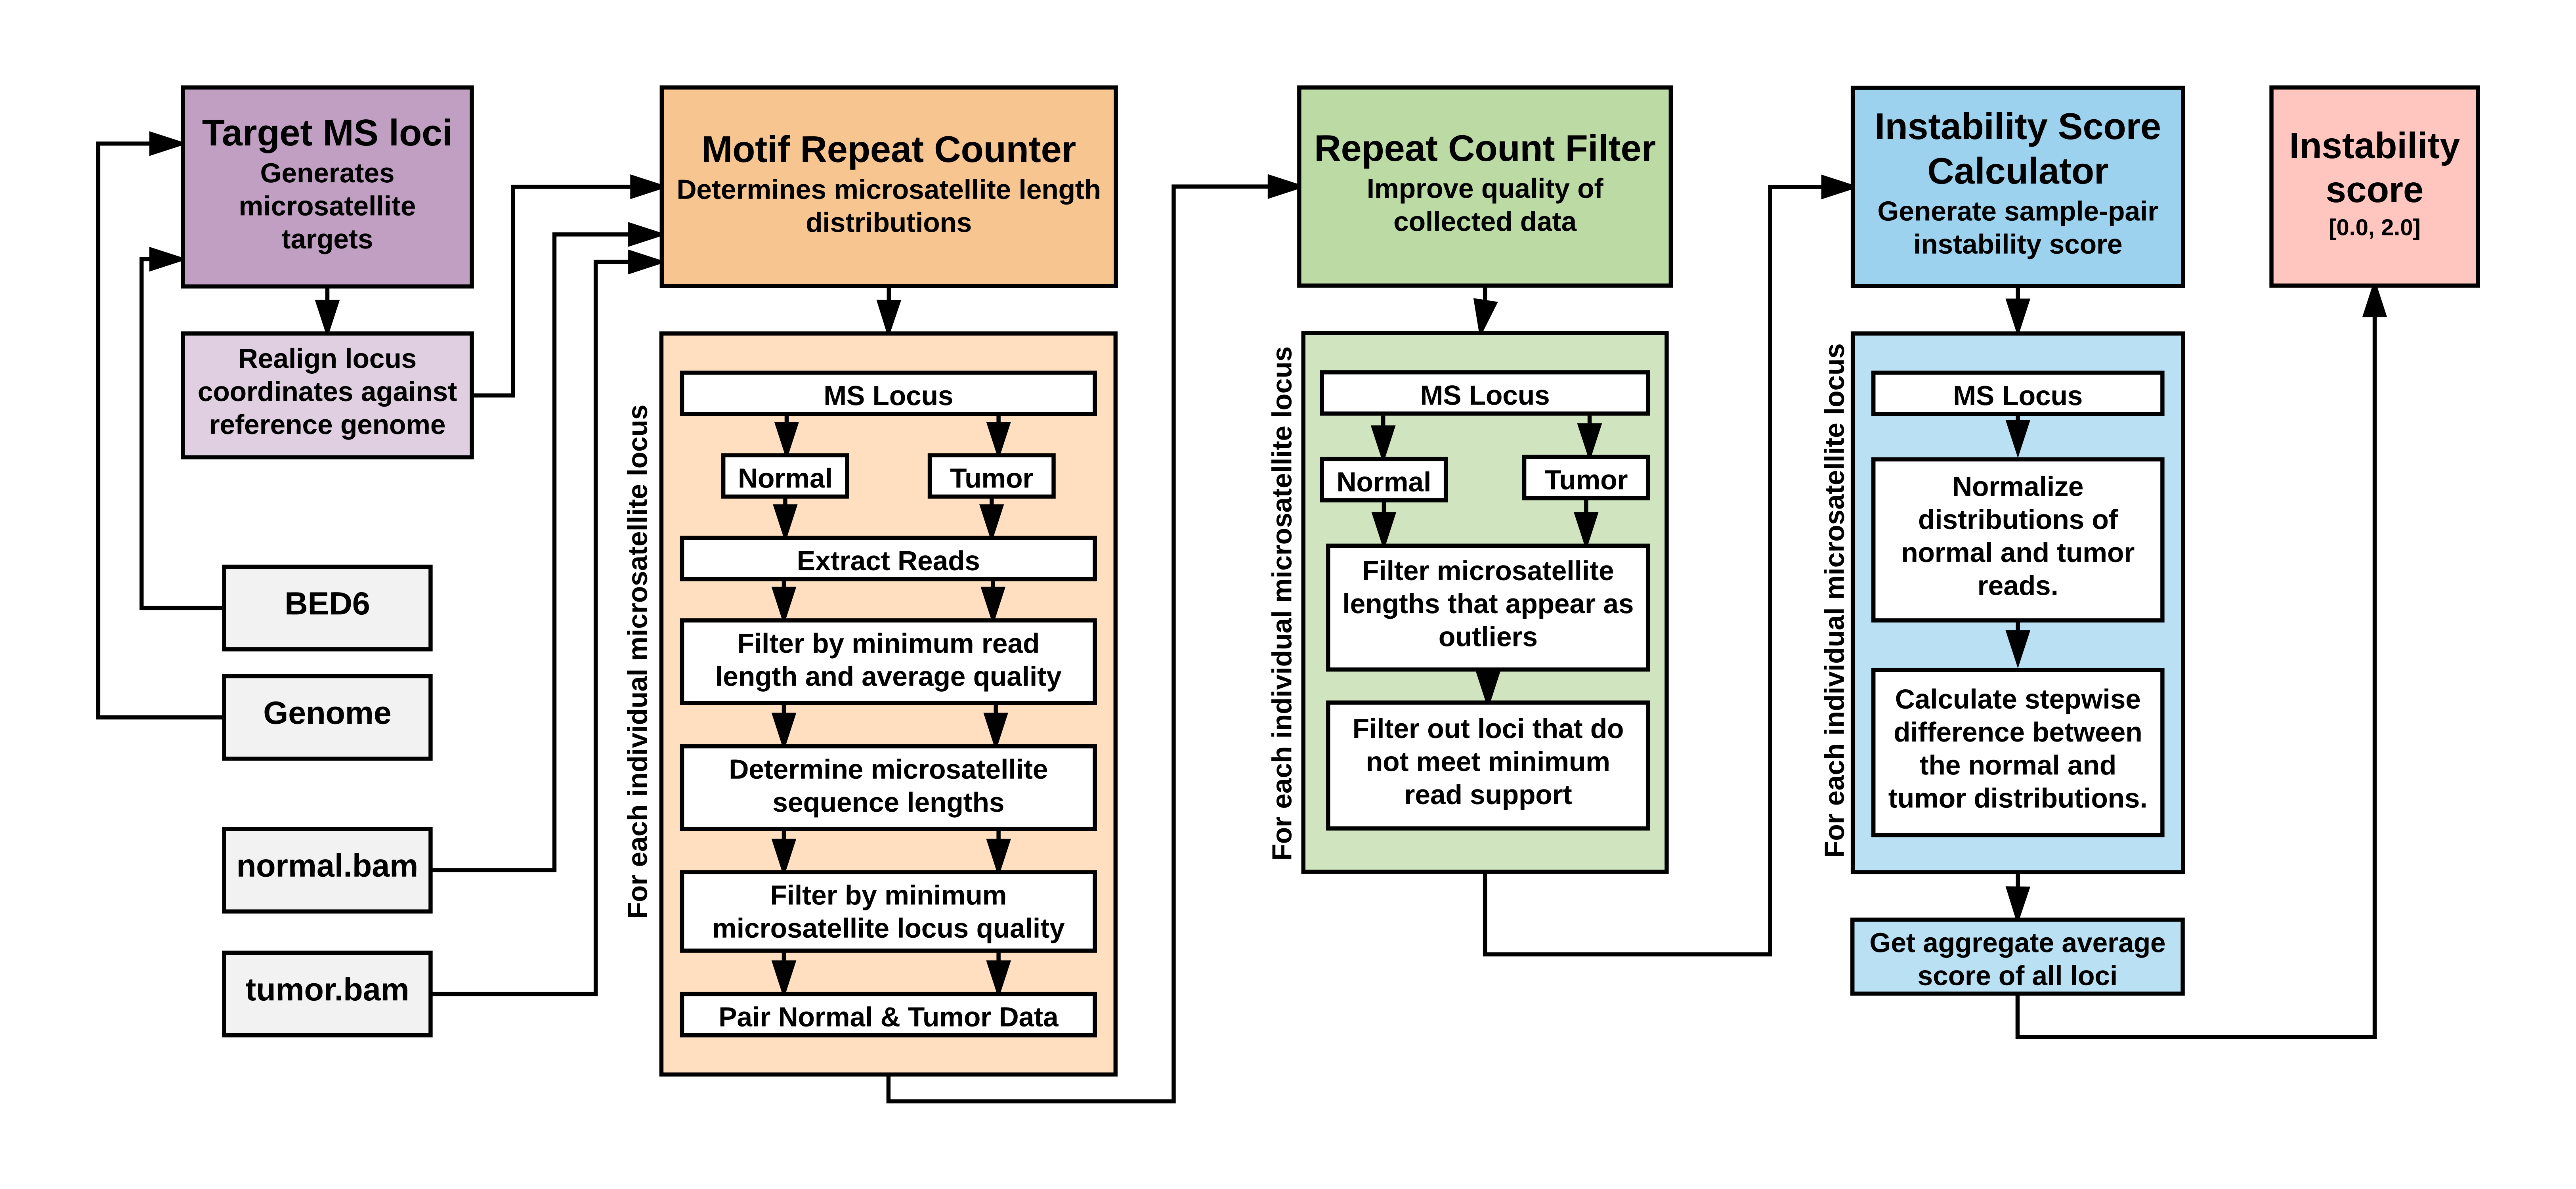
\includegraphics[width=\linewidth,keepaspectratio]{images/msilandscape/mantis_flowchart}
	\caption[Schematic of the MANTIS analysis for MSI detection.]{The schematic of the MANTIS analysis for MSI detection. Microsatellite loci are realigned against the reference genome to account for 0/1-based indexing differences. Per-locus microsatellite length distributions are determined from the normal and tumor BAM files by extracting locus-spanning reads; filtering out reads that fail to meet minimum length and average base quality requirements; determining the start position of the microsatellite motif within each read's sequence and the number of motif repeats; ensuring such reads meet minimum average locus quality and are not prematurely truncated in the middle of a motif repeat. The generated normal and tumor length distributions are evaluated at each locus, with outlying length values (by default, \textgreater{}~3~SD from mean) removed. Loci with substandard coverage are also removed. The support counts at each locus are then normalized separately for the normal and tumor sample and the stepwise difference between each distribution is calculated. Finally, the average of all difference scores is taken to generate the instability score for the normal-tumor sample pair.}
	\label{fig:msilandscape:mantis_flowchart}
\end{figure}
MANTIS is a tool for identifying microsatellite instability in paired tumor-normal patient samples (Figure~\ref{fig:msilandscape:mantis_flowchart}). It is written as a Python program, utilizing the NumPy (developed with version 1.6.2) \cite{2020NumPy-Array} and Pysam (developed with version 0.8.3) \cite{samtools} libraries. Additionally, it requires the reference genome in FASTA format to perform alignment of reads spanning the microsatellite loci. The matched normal and tumor inputs are required as indexed BAM files, aligned with any DNA sequence aligner. The targeted loci are required in a 6-column BED file, with the fourth column containing the motif of the microsatellite loci being targeted along with its repeat count in the reference genome, \textit{e.g.}\ \texttt{(AC)12}. MANTIS includes a bundled C\texttt{++} program, RepeatFinder, used to identify microsatellite loci within a reference genome, and create the appropriate BED file. This BED file can be further filtered with BEDTools \cite{quinlan2010} for regions of interest. Multi-threading is supported and encouraged for larger samples, but is not necessary. More information about the parameters supported by MANTIS is included in the manual available with the software.

Targeted loci are first read from the provided BED file and realigned against the provided reference genome to account for differences between 0- and 1-based indexing. One locus at a time, the tool extracts overlapping reads from the tumor and normal BAM files and performs an initial quality control step to ensure the reads are of sufficient sequence length, meet a minimum average base quality score, and cover the entire targeted locus. Reads passing the initial filtering step are inspected individually to determine the starting position of the microsatellite motif within the read's sequence and the total number of repeats is determined by pattern matching the continuous motif pattern from that starting point. Once the repeat count is determined, a secondary quality control step takes place, ensuring that the locus was not truncated before reaching the end of the read's sequence, and that the microsatellite locus region has a sufficiently high average base quality score. The supporting read count for each of the repeat lengths is determined separately for the tumor and normal files to generate per-locus motif repeat count values.

Once the repeat counts are generated for each locus, a per-locus quality control step takes place. The repeat lengths for both the normal and tumor file are evaluated separately, with values too far from the mean (by default, beyond 3 standard deviations) discarded as outliers. After outliers are removed, each locus is checked for a total number of supporting reads to ensure there is sufficient support to generate a statistically significant distribution for both the normal and tumor files. Loci with substandard coverage are discarded. 

The filtered locus repeat count data is then passed to the scoring algorithm that generates an instability score for the sample pair. First, each locus is evaluated separately, with the normal and tumor read distributions normalized to a fraction of each one's total reads, to account for any differences in sequencing depth and coverage. Then, absolute value of the stepwise difference between the tumor and normal distributions is determined:
\begin{equation}
	d=\sum_{r \in (R_T \cup R_N)} \left|T_r - N_r\right|
	\label{eqn:msilandscape:mantis_sum}
\end{equation}
where $d$ = distance score, $R_T$ = repeat counts present in tumor, $R_N$ = repeat counts present in normal, $T_r$ = normalized read count in tumor supporting repeat of length $r$, $N_r$ = normalized read count in normal supporting repeat of length $r$. Once the scores for each locus are assigned, the average of all the locus instability scores is calculated, to provide a single numerical value representing the average aggregate instability present in the sample. Scores reported range from 0.0 (entirely stable) to 2.0 (entirely unstable). The MANTIS software and manual are freely available for download at \url{https://github.com/OSU-SRLab/MANTIS}.

\subsection{Comparison of tools}
\begin{table}[H]
	\begin{center}
		\begin{tabular}{l|c|c|c}
			\textbf{Tool} & \textbf{Sample Comparison} & \textbf{Statistical Method} & \textbf{Scoring Approach} \\
			\hline
			\textbf{mSINGS} & Tumor vs.\ Baseline & Z-score & Per Locus \\
			\textbf{MSISensor} & Tumor vs.\ Normal & Chi-square & Per Locus \\
			\textbf{MANTIS} & Tumor vs.\ Normal & Average distance & Aggregate Instability
		\end{tabular}
	\end{center}
	\vspace{-0.3cm}
	\caption[Comparison of the MSI-calling tools mSINGS, MSISensor and MANTIS.]{Comparison of the MSI-calling tools mSINGS, MSISensor and MANTIS, and the algorithms used by each.}
	\label{table:msilandscape:tool_comparison}
\end{table}
In addition to MANTIS, we tested mSINGS (commit \verb|#2e00b6|) by Salipante \textit{et al} \cite{salipante2014} and MSISensor (version 0.2) by Niu \textit{et al} \cite{niu2013} (Table~\ref{table:msilandscape:tool_comparison}). mSINGS compares a tumor sample to a pooled normal baseline, generated from the distribution of unique alleles at each microsatellite locus in many normal samples. MSISensor, like MANTIS, compares a tumor sample with its matched normal sample. Both mSINGS and MSISensor determine the stability of each locus analyzed. mSINGS calls a locus unstable if the Z-score of the number of unique alleles at the locus relative to the baseline distribution exceeds a threshold (default: 2). MSISensor calls a locus unstable if a chi-square test of the repeat lengths in the tumor sample vs.\ the normal sample is statistically significant, after Benjamini correction for multiple hypotheses \cite{benjamini1995}. Both tools then call the sample MSI-H or MSS if the percentage of unstable loci exceeds a threshold.

\subsection{Tool parameters}
\label{ssec:msilandscape:tool_params}
mSINGS was run with Python 2.7.1, VarScan 2.3.6 \cite{varscan2} and SAMtools 0.1.18 \cite{samtools}. The wrapper script provided with mSINGS was modified to remove its dependency on SCons (\url{http://scons.org/}). We generated separate pooled normal baselines from all normal samples within a particular cancer type, according to the mSINGS documentation. The microsatellite loci-containing region BED and .intervals files packaged with mSINGS were used, which contained 2,539 loci, as they are appropriate for whole exome TCGA analyses according to the mSINGS documentation.

MSISensor was slightly modified to output sites that were not called with somatic microsatellite instability along with its other output files, and compiled from source. It was run over the test data with the following settings: single-threaded, minimal homopolymer size 1, and minimal microsatellite size 1. All other options were left at their defaults. The microsatellite loci-containing region BED file packaged with mSINGS was used for fairness of comparison, as well as to restrict MSISensor to exomic regions.

MANTIS was run over the test data with three threads. The recommended quality settings for whole exome data were used as described in the included MANTIS manual; min read quality 20, min locus quality 25, and min read length 35. The microsatellite BED file was derived from the one provided by mSINGS\@.

\subsection{Target loci selection}
\label{ssec:msilandscape:loci_selection}
\begin{table}[H]
	\begin{center}
		\begin{tabular}{l|r|r|r|r}
			\textbf{Type of} & \textbf{Number of} & \textbf{Min Repeats} & \textbf{Max Repeats} & \textbf{Mean Repeats} \\
			\textbf{Microsatellite} & \multicolumn{1}{l|}{\textbf{Loci}} & & & \\
			\hline
			Monomer & 2436 & 3 & 36 & 15.94 \\
			Dimer & 96 & 6 & 18 & 14.86 \\
			Trimer & 4 & 3 & 8 & 4.75 \\
			Tetramer & 2 & 7 & 8 & 7.5 \\
			Pentamer & 1 & 3 & 3 & 3
		\end{tabular}
	\end{center}
	\vspace{-0.3cm}
	\caption[Breakdown of target loci used for microsatellite status calling.]{Breakdown of target loci used for microsatellite status calling. The count and repeat range of each type is listed.}
	\label{table:msilandscape:target_loci}
\end{table}
The 2,539 target loci being analyzed were derived from the ones provided with mSINGS and captured in whole exome sequencing data sets, and used with all three tools. Most of the targeted loci (Table~\ref{table:msilandscape:target_loci}) were monomer homopolymers of adenine or thymine (95.08\%), with only 4.04\% of loci being repeats of dimers or longer polymers. This bias towards monomer repeats was expected since intronic mononucleotide repeats outnumber other repeat regions in the human genome \cite{toth2000}. 

\subsection{Testing data}
\label{ssec:msilandscape:testing_data}
To evaluate mSINGS, MSISensor, and MANTIS, we used data from six cancer types: 76 colon and rectal adenocarcinomas (COAD/READ) \cite{tcgacoadread}, 99 uterine corpus endometrial carcinomas (UCEC) \cite{tcgaucec}, 100 gastric adenocarcinomas (STAD) \cite{tcgastad}, 71 esophageal carcinomas (ESCA), 53 uterine carcinosarcomas (UCS) \cite{tcgageneric}, and 59 prostate adenocarcinomas (PRAD) \cite{robinson2015}. Cancer type abbreviations are listed in Appendix~\ref{app.cancerabbrev}. We define a ``sample'' as a single BAM and its accompanying BAI index file, for a tumor or a normal. We define a ``pair'' as two samples; a tumor and its matched normal, and define a ``cohort'' as all samples within a cancer type, for a total of 6 cohorts (Table~\ref{table:msilandscape:test_samples_count}).

Data for all cohorts except PRAD were downloaded from the Cancer Genomics Hub (CGHub), using the CGHub-provided client GeneTorrent \cite{wilks2014}. All samples were downloaded in the BAM format, pre-aligned to GRCh37/hg19 \cite{lander2001}. 76 COAD/READ pairs were downloaded, comprised of 38 MSI-H and 38 MSS\@. COAD/READ data was sequenced at the Baylor College of Medicine (BCM) and the Washington University Genome Sequencing Center (WUGSC) (Table~\ref{table:msilandscape:test_samples_bycenter}). 99 UCEC pairs were downloaded, comprised of 49 MSI-H and 50 MSS\@. All UCEC pairs were sequenced at WUGSC\@. Next, 100 STAD pairs were downloaded; 50 MSI-H and MSS\@. All STAD pairs were sequenced at the Broad Institute of MIT and Harvard (BI)\@. The primary authors were blinded to the MSI status of these samples until after initial analysis with mSINGS, MSISensor and MANTIS was completed. Finally, 71 ESCA pairs were downloaded from TCGA; 2 MSI-H and 69 MSS, and 53 UCS pairs were downloaded; 2 MSI-H and 51 MSS\@. All ESCA and UCS pairs were sequenced at BI\@. PRAD data was downloaded from the Database of Genotypes and Phenotypes (dbGaP) (accession phs000915.v1.p1) \cite{mailman2007} as FASTQ files, using the SRA toolkit \cite{leinonen2010sra}. All 59 available PRAD pairs were downloaded; 1 MSI positive and 58 MSI negative (according to the original study for which these samples were sequenced, which only differentiated between MSI positive and MSI negative). PRAD data was sequenced at BI and the University of Michigan (UM) (Table~\ref{table:msilandscape:test_samples_bycenter}). Alignment to hg19 was performed with with Burrows-Wheeler Aligner (BWA) 0.6.2 \cite{bwa}.

Each of the 916 BAM files (from the 458 tumor-normal pairs in all six cancer types) were sorted and indexed with SAMtools 0.1.18. Deduplication was performed with Picard Tools 1.84 \cite{Picard2019toolkit}, and facilitated with GNU Parallel \cite{tange2011}. The deduplicated BAM files were used for all downstream analyses. Samples used in these analyses are summarized in Supplemental File~S\thechapter{}.1.

\subsection{Tool performance evaluation}
mSINGS, MSISensor and MANTIS were first run on all 175 tumor-normal pairs from COAD/READ and UCEC (Supplemental File~S\thechapter{}.2). A threshold was used for each tool, above which a tumor-normal pair is called MSI positive. For mSINGS, 0.2 (20\% of loci called unstable) was used as the threshold for differentiation of MSI positive from MSS predictions, as this is consistent with both MSI-PCR scoring and the threshold used by Salipante \textit{et al}. A threshold of 3.5\% (of loci called unstable) was used for MSISensor, as recommended by Niu \textit{et al}. For MANTIS, a threshold of 0.4 (average of loci difference scores \textgreater{}~0.4) performed best in testing (Section~\ref{ssec:msilandscape:tool_accuracy}), and was used for other analyses. For each tool, the number of true positives, false positives, true negatives, and false negatives was calculated with respect to MSI-PCR status as a gold standard, and this was used to calculate the sensitivity, specificity, error rate, and accuracy of each tool both overall and within each cancer type. Error rate was calculated as $\text{incorrect calls} / \text{total calls}$, and accuracy as $1-\text{error rate}=\text{correct calls} / \text{total calls}$. Note that error rate and accuracy depend on the samples being tested, and cannot be generalized to other data sets, as can sensitivity and specificity. 95\% confidence intervals for sensitivity and specificity were calculated using the Wilson score interval with continuity correction \cite{newcombe1998}. In addition, ranges of thresholds were tested for all three tools in order to determine which thresholds provided optimal performance with the COAD/READ and UCEC test data, allowing comparison of best-case performance. 300 thresholds ranging from 0.001 to 0.3 were tested for mSINGS, 400 thresholds ranging from 0.1\% to 40\% were tested for MSISensor, and 600 thresholds ranging from 0.001 to 0.6 were tested for MANTIS\@. After a threshold of 0.4 was chosen for MANTIS, we ran mSINGS, MSISensor and MANTIS over the 100 STAD, 71 ESCA, 53 UCS and 59 PRAD tumor-normal pairs. Tool parameters were selected and performance analyses were performed as described earlier.

For each tool, we measured potential bias arising from differences in sequencing and alignment protocols at different sequencing centers. In addition to the sample data used for tool performance comparison, TCGA data from 4 tumor-normal COAD/READ MSI-H pairs sequenced at both BI and BCM, as well as from 20 tumor-normal UCEC MSI-H pairs sequenced at both BI and WUGSC, was downloaded and preprocessed as earlier (Section~\ref{ssec:msilandscape:testing_data}) (Supplemental File~S\thechapter{}.3). After deduplication, these pairs were analyzed with mSINGS, MSISensor and MANTIS\@. MSISensor and MANTIS were run with the parameters described earlier (Section~\ref{ssec:msilandscape:tool_params}). For mSINGS, the normal BAM files were used to generate separate baselines for each cancer type and sequencing center.

In addition to evaluating the statistical performance of each tool, we also evaluated their computational performance. All three tools were profiled with the runtime and memory usage metrics supplied by the PBS (Portable Batch System) cluster queueing system. MSISensor and MANTIS were tested with one and three threads to evaluate changes in performance (mSINGS does not support multithreading).

\subsection{Loci number comparison}
\label{ssec:msilandscape:loci_number_comparison}
For each of the three tools tested, the top-performing 10, 20, 30, 40, 50, 100, 250, 500 and 1000 microsatellite loci within the COAD/READ, UCEC and STAD samples were determined, individually within each cancer type and across all three cohorts. ESCA, UCS and PRAD were not included in this as only five MSI-H cases were available from these cancer types. To determine the top $n$ loci for mSINGS and MSISensor, the accuracy of each locus was calculated as if only that locus were to be used to call the MSI status of each tumor sample. For MANTIS, since it calculates instability scores instead of assigning per-locus stability statuses, a difference of averages was calculated for each locus, defined as:
\begin{equation}
	a = \frac{\sum_{i \in H} d_i}{\left|H\right|} - \frac{\sum_{i \in S} d_i}{\left|S\right|}
\end{equation}
where $a$ = difference of averages, $H$ = set of MSI-H samples that cover the locus, $S$ = set of MSS samples that cover the locus, and $d_i$ = distance score of the locus in sample $i$. To compensate for varying locus coverage across samples, this score (accuracy or difference of averages) was then multiplied by the square of the proportion of pairs that had sufficient read coverage at that locus to consider it, as follows:
\begin{equation}
	l = ac^2
\end{equation}
where $l$ = locus score, $a$ = accuracy or difference of averages, and $c$ = proportion of samples that cover the locus. This yielded a performance score for each locus, which allowed all 2,539 loci to be ranked. The sensitivity, specificity, error rate, and accuracy of each tool with each loci list was then calculated, both for all three of these cancer types and overall (Supplemental File~S\thechapter{}.4).

\subsection{Landscape data preprocessing}
\subsubsection{L-MAP: Landscape Microsatellite Analysis Pathway}
\begin{figure}[htp]
	\centering
	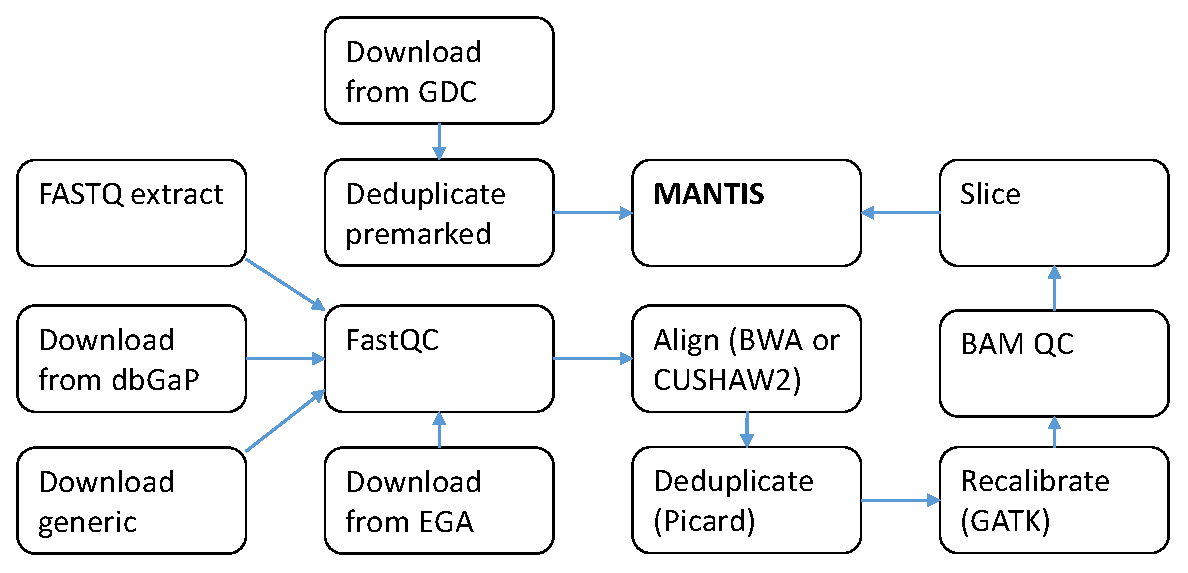
\includegraphics[width=0.8\linewidth,keepaspectratio]{images/msilandscape/lmap_flowchart}
	\caption[Schematic of L-MAP for bulk MSI analysis.]{Schematic of L-MAP (Landscape Microsatellite Analysis Pathway), an automated pipeline developed for bulk calling of microsatellite instability within large genomc data sets.}
	\label{fig:msilandscape:lmap_flowchart}
\end{figure}
To facilitate bulk processing and analysis of microsatellite instability, we developed an in-house automated pipeline, L-MAP (Figure~\ref{fig:msilandscape:lmap_flowchart}). L-MAP is implemented in Python and MySQL\@. L-MAP periodically polls a MySQL database for pending tasks in a pre-specified pipeline, and submits jobs to the PBS scheduler while respecting defined resource limits (concurrent batch jobs, cumulative storage utilization). Task types are specified in a MySQL table, with primary:foreign key pairs used to specify job dependencies. L-MAP supports input from available FASTQ files, along with automated downloads from generic URLs, dbGaP, the Genomic Data Commons (GDC) \cite{grossman2016}, and the European Genome-Phenome Archive (EGA) \cite{lappalainen2015}. QC metrics are computed for acquired FASTQs using FastQC \cite{fastqc}. Alignment is supported using BWA \cite{bwa} for Illumina reads and CUSHAW2 \cite{liu2012} for ABI SOLiD color-space reads (not used in this study). Reads are deduplicated with Picard MarkDuplicates \cite{Picard2019toolkit}, or pre-marked duplicates removed with SAMtools. Quality score recalibration and local realignment of reads around indels are performed with Genome Analysis Toolkit (GATK) \cite{mckenna10}. Additional basic QC measures (such as alignment percentage) are computed, and BAM files are sliced using SAMtools to retain only reads covering microsatellite regions to conserve storage space. Finally, MSI status is computed for tumor-normal sequencing pairs with MANTIS and MSISensor.

\subsubsection{TCGA and TARGET}
10,701 cases of paired tumor-normal whole exome sequencing data were obtained from The Cancer Genome Atlas (TCGA) \cite{tcgacoadread,tcgaucec,tcgastad,tcgaov,tcgabrca,tcgalaml,tcgakirc,tcgagbm,tcgablca,tcgaluad,tcgalusc,hoadley2014,tcgakich,tcgathca,tcgahnsc,tcgalgg,tcgaskcm,ciriello2015,tcgakirp,tcgaprad,tcgaacc,tcgaesca,tcgacesc,tcgapcpg} and Therapeutically Applicable Research to Generate Effective Treatments (TARGET) \cite{target,targetnbl} projects. Data from all of these cases except diffuse large B-cell lymphoma (DLBC) were processed through L-MAP\@. First, the metadata for all DNA whole exome BAM files was downloaded from GDC, and was converted to SQL database entries. Aligned BAM files (to hg38 \cite{lander2001}) were queried from GDC by L-MAP using the slicing endpoint provided by the GDC REST API\@. Reads covering any base within 50 base pairs (bp) of a desired microsatellite locus were downloaded. As GDC data harmonization includes duplicate marking, premarked duplicate reads were removed using SAMtools (version 1.3.1).

Due to a GDC sample contamination issue, all 48 DLBC paired tumor-normal cases were downloaded from the GDC Legacy Archive as whole exome BAM files aligned to hg19, using the GDC Data Transfer Tool, and separately analyzed. Premarked duplicate reads were removed as above.

\subsubsection{Other sources}
430 cases of paired tumor-normal whole exome sequencing data were obtained from the Sequence Read Archive \cite{leinonen2010sra}: 338 chronic lymphocytic leukemia (CLL) cases from 279 patients from Landau \textit{et al} \cite{landau2015}, 32 cutaneous T-cell lymphoma (CTCL) cases from Choi \textit{et al} \cite{choi2015}, 51 nasopharyngeal carcinoma (NPC) cases from Zheng H \textit{et al} \cite{zheng2016}, and 8 cholangiocarcinoma (CHOL) cases from Ong \textit{et al} \cite{ong2012}. 15 additional CHOL cases were obtained from the European Nucleotide Archive \cite{leinonen2010ena}, from Chan-on \textit{et al} \cite{chanon2013}. All sample identifiers used are available in Supplemental File~S\thechapter{}.5. These cases were processed through L-MAP\@. Tumor and normal samples were downloaded in the FASTQ format using fastq-dump \cite{leinonen2010sra}. Alignment to hg38 was performed using BWA (version 0.7.12) \cite{bwa} with the mem algorithm. Duplicate reads were marked and removed using Picard MarkDuplicates. Base quality score recalibration and indel realignment were performed using GATK, and the resulting BAM files were sliced (as above) using SAMtools.

\subsection{MSI calling --- landscape}
MSI analysis with MANTIS (version 1.0.3, commit \#942061f) was performed for all cases, using an average distance threshold of 0.4 to differentiate MSI-H from MSS tumors. The set of 2,539 coordinates within or near the exome used for MANTIS validation (Section~\ref{ssec:msilandscape:loci_selection}) were converted from hg19 to hg38 using UCSC LiftOver \cite{hinrichs2006}. Nine unlifted loci were discarded, leaving 2,530 regions that were used for analysis with MANTIS in all cohorts except DLBC (Supplemental File~S\thechapter{}.6). As the DLBC data was aligned to hg19, the original 2,539 loci were used instead. MANTIS was run with author-recommended settings for whole exome data (Section~\ref{ssec:msilandscape:tool_params}), with all other settings left at defaults. Eight samples were found to have fewer than 10 loci sufficiently covered, and were dropped from further analysis. After MSI calling, microsatellite locus performance was assessed in each cancer type as described above (Section~\ref{ssec:msilandscape:loci_number_comparison}). Kernel density estimation functions were computed using R (version 3.3.2), using the \texttt{density()} function with default settings.

\subsection{Whole exome analysis}
For all tumor-normal pairs tested by MANTIS in ACC (n = 92), CESC (n = 305), and MESO (n = 83), we downloaded aligned reads from whole exome sequencing. Reads were downloaded in BAM format from GDC, using the GDC Data Transfer Tool. Premarked duplicate reads were removed using SAMtools, variant calling was performed using MuTect \cite{cibulskis2013}, and annotation was performed using ANNOVAR \cite{annovar} (version 2016-02-01) and GNU Parallel.

\subsection{Variant calling}
\label{ssec:msilandscape:variant_calling}
All variant calling was performed using MuTect version 1.1.7. The target region was derived from RefSeq \cite{oleary2015} release 80. Exon data from the refGene table of the RefSeq Genes track was downloaded in BED format on February 28, 2017, using the UCSC Table Browser \cite{karolchik2004} and 100 bp padding. Unknown contigs were excluded, and overlapping regions were merged with BEDTools. VCF output was specified for MuTect, and all other options were left at their defaults. MuTect VCF output was then filtered for variants marked PASS\@. Variant annotation was performed using ANNOVAR and GNU Parallel. Somatic mutations in the DNA repair genes \textit{MSH2}, \textit{MSH6}, \textit{MLH1}, \textit{PMS2}, \textit{EXO1}, \textit{POLD1}, and \textit{POLE} were determined by filtering variants with a DANN \cite{quang2015} pathogenicity score above 0.96 (included in ANNOVAR)\@. This threshold for DANN was chosen as it was previously shown to provide optimal sensitivity and specificity \cite{jensen2015}.

Mutational signature calling was performed using the tool deconstructSigs \cite{rosenthal16}, with the Nature 2013 signatures set (containing 27 signatures) \cite{alexandrov2013} and ``exome2genome'' normalization method. A mutational signature is a probability vector of length 96, with each element representing a single base change, along with the bases immediately flanking it. In this analysis, non-negative linear regression is used to determine the relative contribution of each signature to the observed pattern of mutations. deconstructSigs was run over every ACC, CESC, and MESO sample, using all passing variants called with MuTect.

\subsection{Computing resources}
Alignment, deduplication, MSI calling with all three tools, tool performance calculations, and all landscape analyses (including L-MAP) were performed on the Oakley supercomputer at the Ohio Supercomputer Center \cite{Oakley2012}. Figures were generated using GraphPad Prism\textsuperscript\textregistered{} and Microsoft\textsuperscript\textregistered{} Excel\textsuperscript\texttrademark{} 2010. All other calculations were performed with custom Perl and Python scripts, R, and Excel\textsuperscript\texttrademark{}.

\section{Results}
\subsection{Evaluation of tool accuracy for detecting MSI status}
\label{ssec:msilandscape:tool_accuracy}
\begin{figure}[htp]
	\centering
	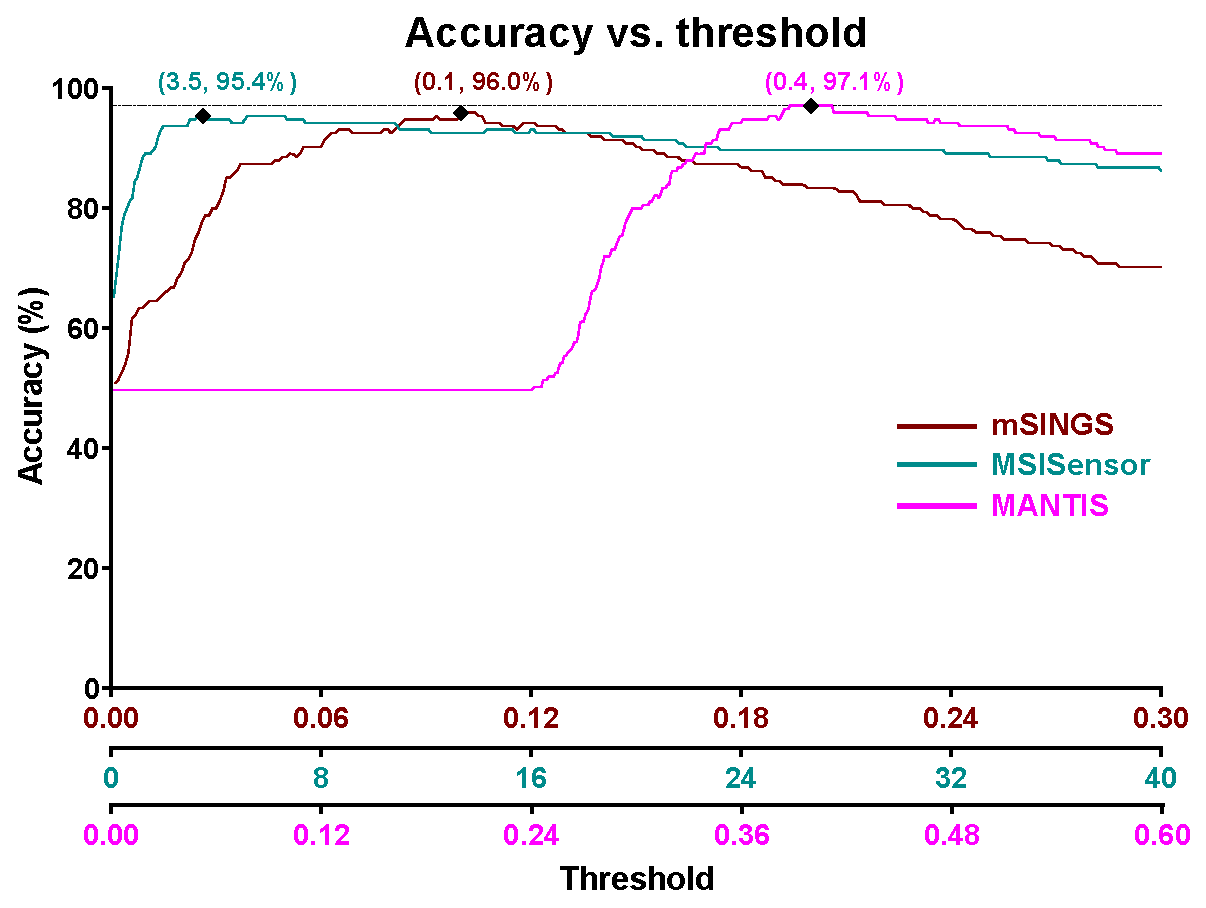
\includegraphics[width=\linewidth,keepaspectratio]{images/msilandscape/tool_thresholding}
	\caption[Accuracy of mSINGS, MSISensor and MANTIS at a range of thresholds.]{Accuracy of mSINGS, MSISensor and MANTIS at a range of thresholds, when tested with the 76 COAD/READ tumor-normal pairs and 99 UCEC tumor-normal pairs. The thresholds for each tool yielding the highest accuracy for the test data are highlighted. For mSINGS, thresholds from 0.001 to 0.3 were evaluated, in increments of 0.001. For MSISensor, thresholds from 0.1 to 40.0 were evaluated, in increments of 0.1. For MANTIS, thresholds from 0.001 to 0.6 were evaluated, in increments of 0.001.}
	\label{fig:msilandscape:tool_thresholding}
\end{figure}
Since mSINGS and MSISensor were each developed on data from single disease cohorts (COAD/READ for mSINGS, UCEC for MSISensor), the two cohorts were used for tool performance comparisons. To account for the possibility of suboptimal recommended cutoff thresholds for each of the three tools, we tested a range of thresholds for each tool across a test cohort consisting of both the COAD/READ and UCEC sample pairs (Figure~\ref{fig:msilandscape:tool_thresholding}). The peak performances of each tool were determined, with MANTIS having 97.1\% accuracy with the default threshold of 0.4, mSINGS reaching 96\% accuracy with a threshold of 0.1, and MSISensor peaking at 95.4\% accuracy with the threshold of 3.5\%. The results indicate that MANTIS demonstrated superior performance over the other tools, even after accounting for the best-case thresholds of the tools.

\begin{figure}[htp]
	\centering
	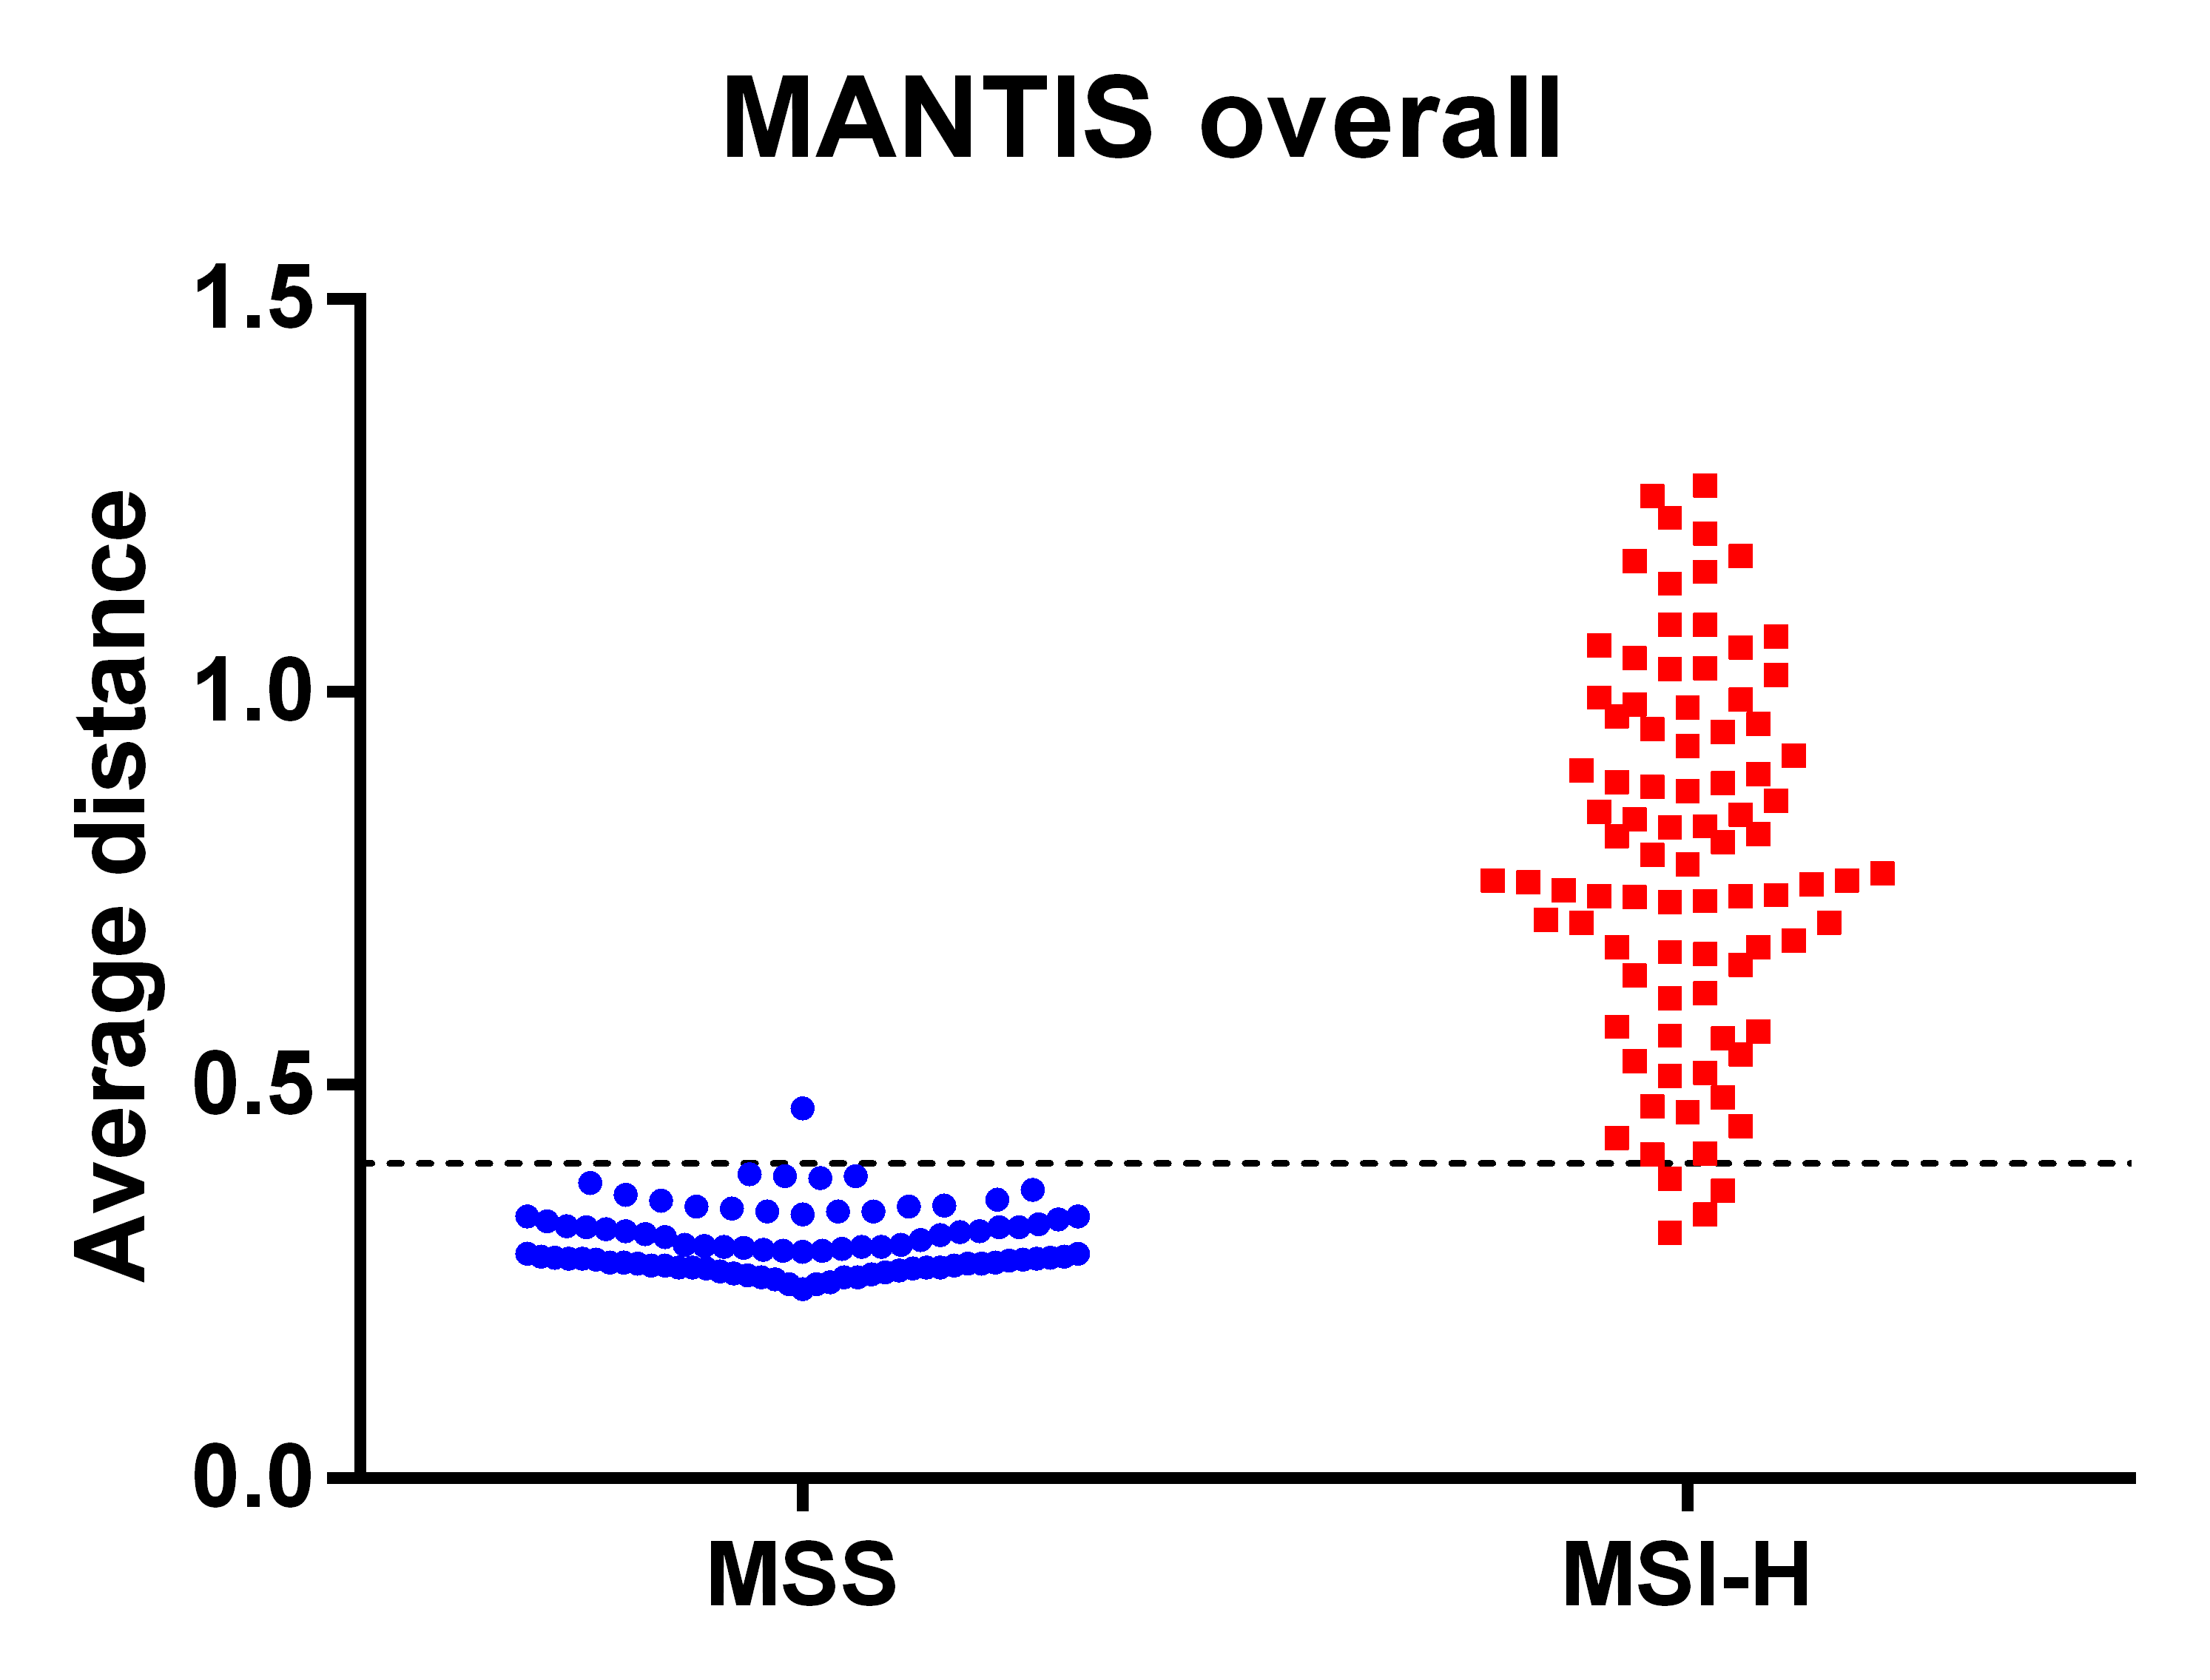
\includegraphics[width=0.5\linewidth,keepaspectratio]{images/msilandscape/mantis_coad_read_ucec}
	\caption[Distribution of MANTIS scores for COAD/READ and UCEC combined tumor-normal pairs.]{The distribution of MSI scores reported by MANTIS for the combined cohorts of 76 COAD/READ tumor-normal pairs and 99 UCEC tumor-normal pairs. The dotted line is at the threshold (0.4) to call a tumor MSI positive.}
	\label{fig:msilandscape:mantis_coad_read_ucec}
\end{figure}
Having evaluated the tools with the best-case thresholds, their performances were evaluated with the tool's recommended default cutoff thresholds (MANTIS 0.4, mSINGS 0.2, and MSISensor 3.5\%) (Figure~\ref{fig:msilandscape:mantis_coad_read_ucec}). MANTIS demonstrated the highest classification accuracy (97.1\%), followed by MSISensor (95.4\%), and mSINGS (83.4\%). MANTIS and MSISensor both exhibited equally high sensitivity (95.4\%). In contrast, although mSINGS was the most specific (100\%), it demonstrated poor sensitivity (66.7\%), largely due to poor performance over the UCEC cohort (53.1\% sensitivity). MANTIS also exhibited high specificity (98.9\%), performing better than MSISensor (95.5\%).

\begin{figure}[htp]
    \centering
    \begin{subfigure}{0.8\textwidth}
        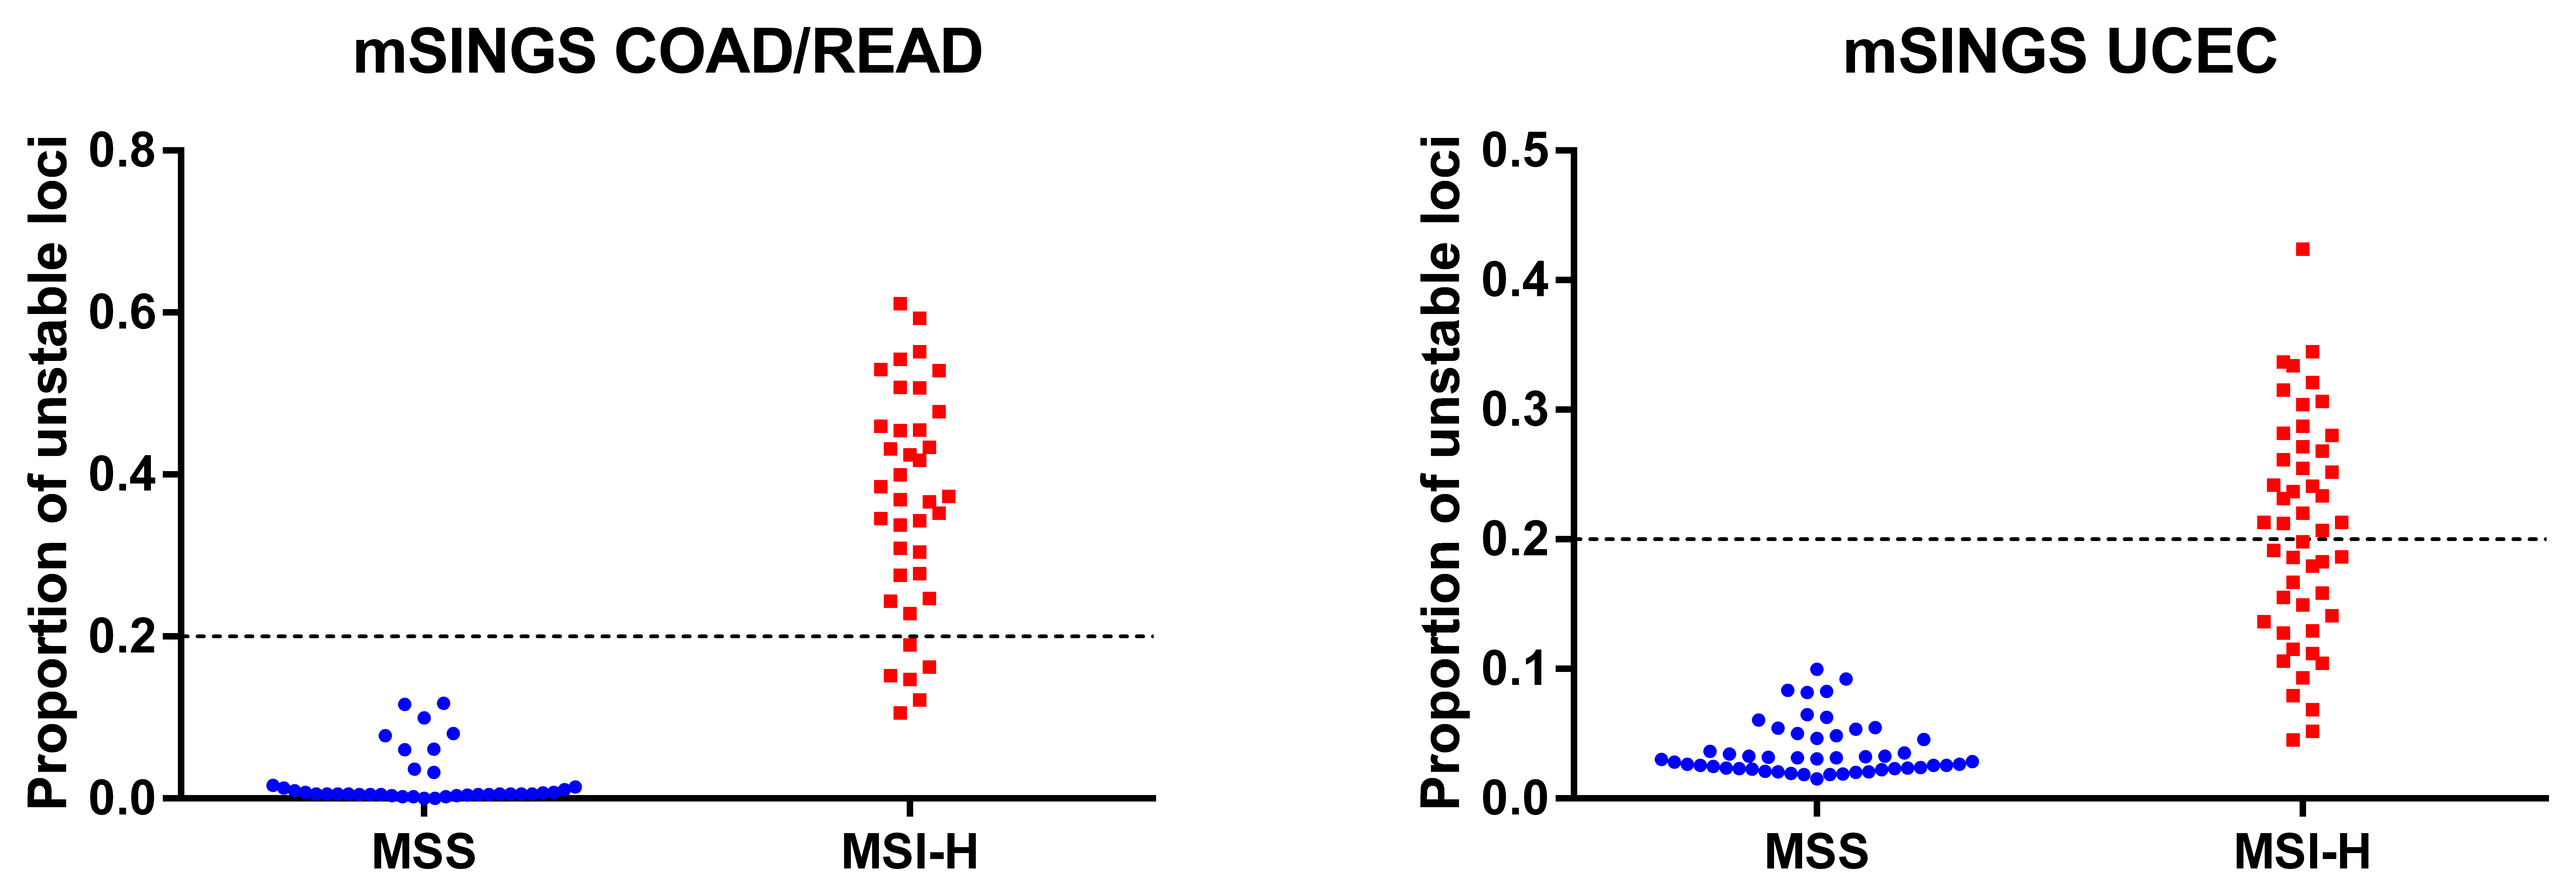
\includegraphics[width=\textwidth,keepaspectratio]{images/msilandscape/perf_coadread_ucec_msings}
        \caption{}\label{fig:msilandscape:perf_coadread_ucec_msings}
    \end{subfigure}\par
    \begin{subfigure}{0.8\textwidth}
        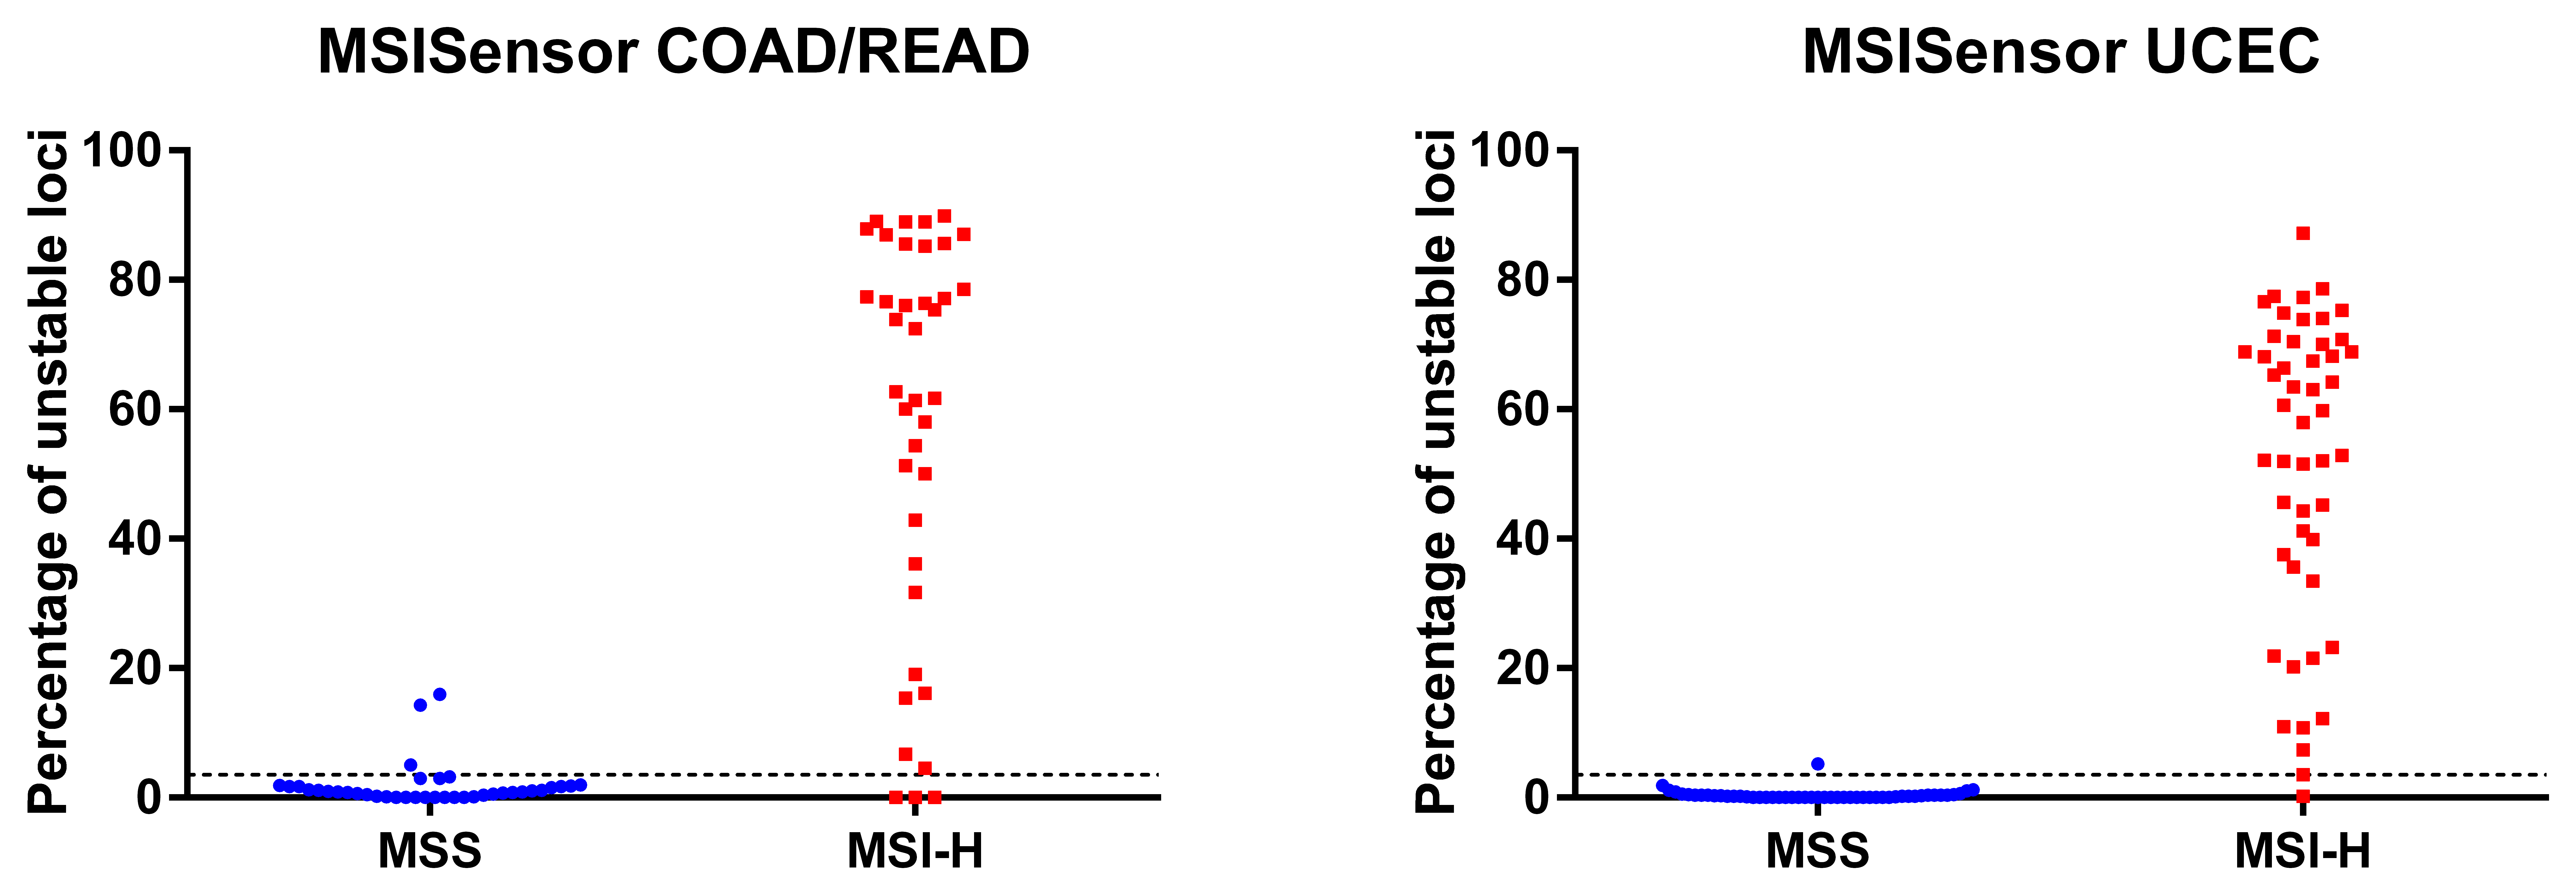
\includegraphics[width=\textwidth,keepaspectratio]{images/msilandscape/perf_coadread_ucec_msisensor}
        \caption{}\label{fig:msilandscape:perf_coadread_ucec_msisensor}
    \end{subfigure}\par
    \begin{subfigure}{0.8\textwidth}
        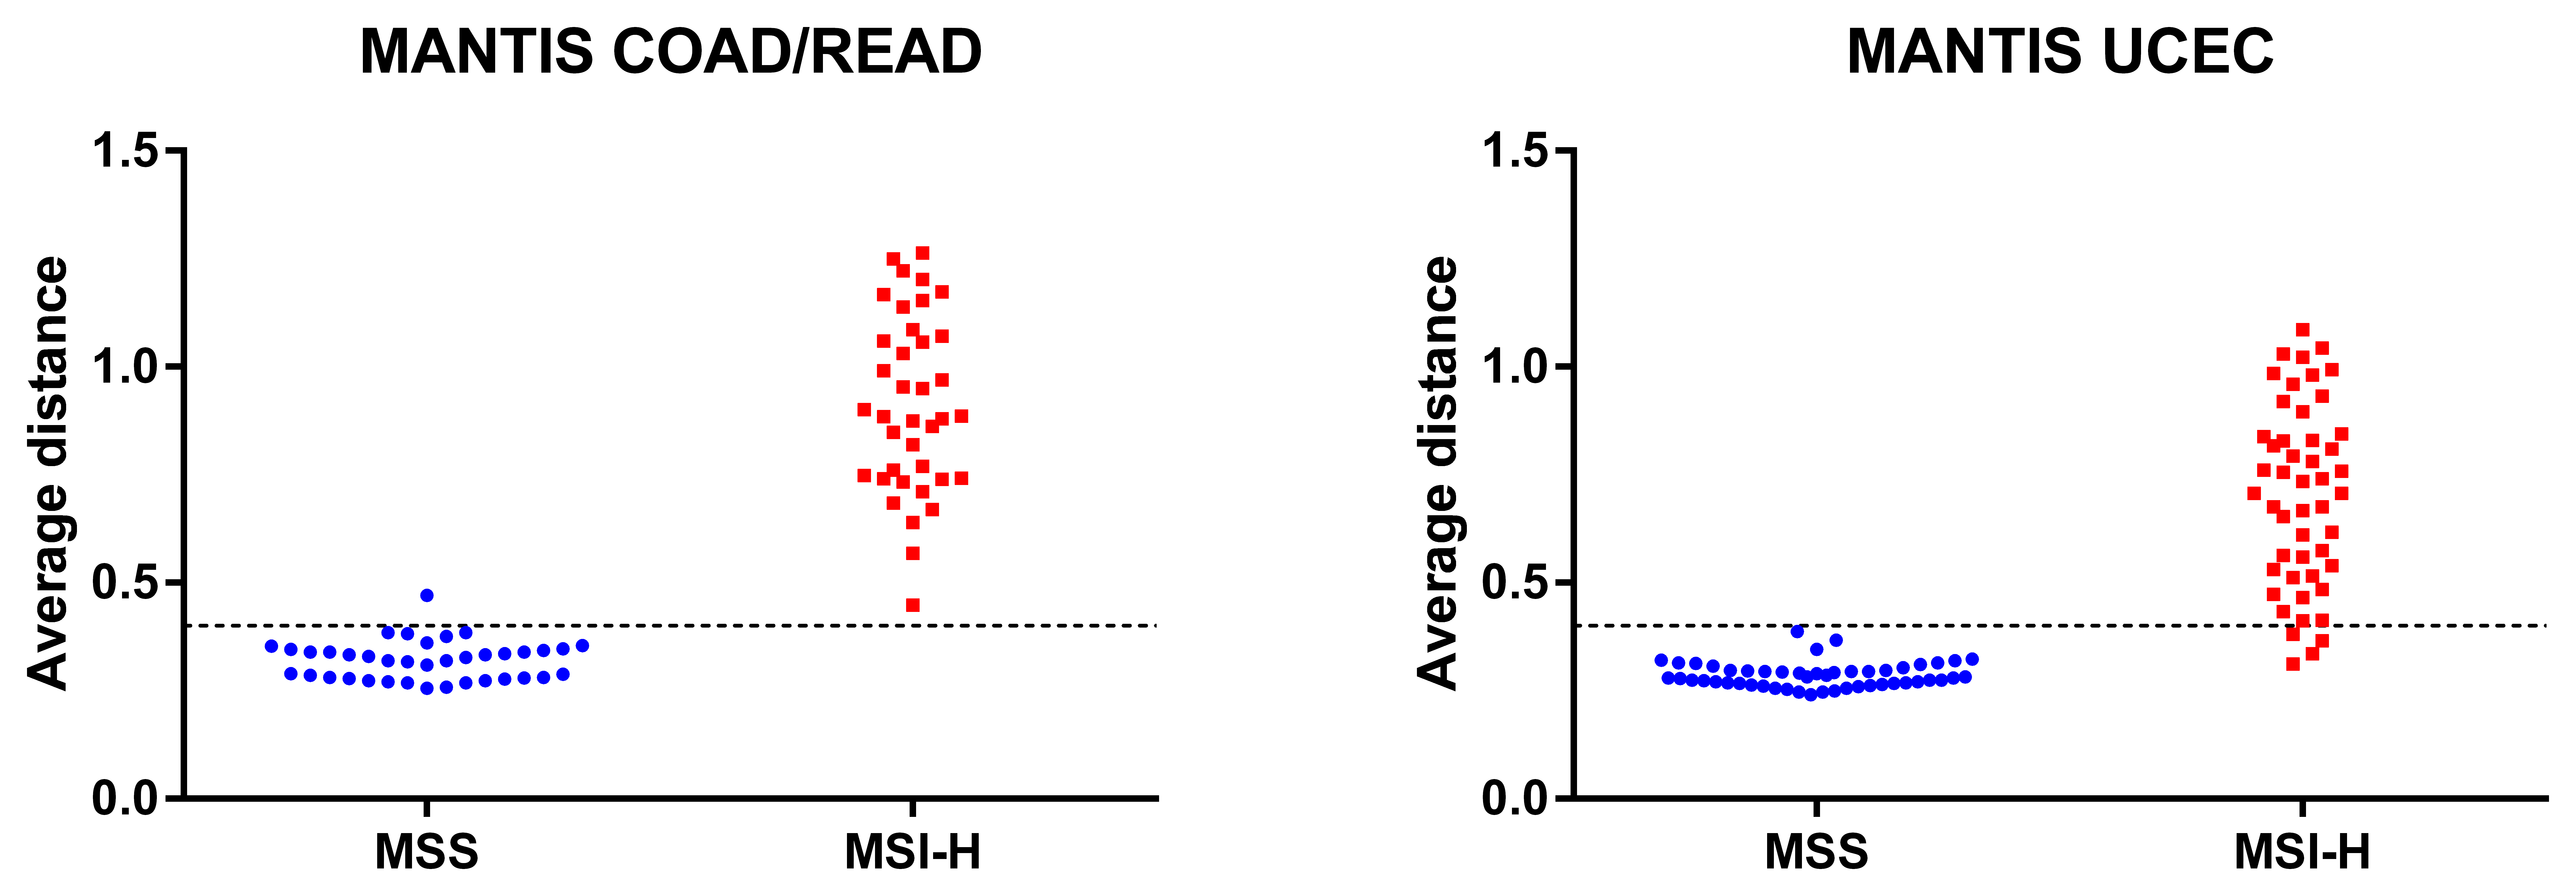
\includegraphics[width=\textwidth,keepaspectratio]{images/msilandscape/perf_coadread_ucec_mantis}
        \caption{}\label{fig:msilandscape:perf_coadread_ucec_mantis}
    \end{subfigure}
    \caption[Distribution of MSI scores from all three tools in COAD/READ and UCEC.]{The cumulative distribution of MSI scores reported by mSINGS (\subref{fig:msilandscape:perf_coadread_ucec_msings}), MSISensor (\subref{fig:msilandscape:perf_coadread_ucec_msisensor}), and MANTIS (\subref{fig:msilandscape:perf_coadread_ucec_mantis}) for the 76 COAD/READ tumor-normal pairs and 99 UCEC tumor-normal pairs. The dotted lines are at the tools' respective thresholds to call a tumor MSI positive.}
    \label{fig:msilandscape:perf_coadread_ucec}
\end{figure}
To analyze disease-specific differences, results were compared between the COAD/READ and UCEC cohorts (Table~\ref{table:msilandscape:tool_accuracy}, Figure~\ref{fig:msilandscape:perf_coadread_ucec}). MANTIS produced more accurate results (98.7\%) than mSINGS (92.1\%) and MSISensor (92.1\%) in COAD/READ, whereas MSISensor was slightly more accurate (98.0\%) than MANTIS (96.0\%) in UCEC\@. While all three tools performed well with the COAD/READ data, mSINGS performed poorly with the UCEC data (accuracy 76.8\%, sensitivity 53.1\%). The tests showed that MANTIS had the most consistently accurate performance among the test cohort, exhibiting high sensitivity (95.4\%) and specificity (98.9\%) among the tested samples.

\subsection{Consideration of data overfitting and bias}
\begin{table}[H]
	\begin{center}
		\begin{tabular}{l|l|l|l|l}
			\multicolumn{5}{c}{\textbf{mSINGS}} \\
			\hline
			\textbf{Metric} & \textbf{COAD/READ} & \textbf{UCEC} & \textbf{COAD/READ} & \textbf{STAD} \\
			& & & \textbf{\& UCEC} & \\
			\textbf{Sensitivity} & 84.2\% & 53.1\% & 66.7\% & 92.0\% \\
			\textbf{Specificity} & 100.0\% & 100.0\% & 100.0\% & 100.0\% \\
			\textbf{Accuracy} & 92.1\% & 76.8\% & 83.4\% & 96.0\% \\
			\hline\hline
			\multicolumn{5}{c}{\textbf{MSISensor}} \\
			\hline
			\textbf{Metric} & \textbf{COAD/READ} & \textbf{UCEC} & \textbf{COAD/READ} & \textbf{STAD} \\
			& & & \textbf{\& UCEC} & \\
			\textbf{Sensitivity} & 92.1\% & 98.0\% & 95.4\% & 98.0\% \\
			\textbf{Specificity} & 92.1\% & 98.0\% & 95.5\% & 100.0\% \\
			\textbf{Accuracy} & 92.1\% & 98.0\% & 95.4\% & 99.0\% \\
			\hline\hline
			\multicolumn{5}{c}{\textbf{MANTIS}} \\
			\hline
			\textbf{Metric} & \textbf{COAD/READ} & \textbf{UCEC} & \textbf{COAD/READ} & \textbf{STAD} \\
			& & & \textbf{\& UCEC} & \\
			\textbf{Sensitivity} & 100.0\% & 91.8\% & 95.4\% & 100.0\% \\
			\textbf{Specificity} & 97.4\% & 100.0\% & 98.9\% & 100.0\% \\
			\textbf{Accuracy} & 98.7\% & 96.0\% & 97.1\% & 100.0\% \\
			\hline\hline
		\end{tabular}
	\end{center}
	\vspace{-0.3cm}
	\caption[Comparison of tool accuracy for MSI-H detection.]{Comparison of tool accuracy for MSI-H detection. The performance of mSINGS, MSISensor, and MANTIS over 275 COAD/READ, UCEC, and STAD sample pairs.}
	\label{table:msilandscape:tool_accuracy}
\end{table}

\begin{figure}[htp]
	\centering
	
\includegraphics[width=0.95\linewidth,keepaspectratio]{images/msilandscape/scores_dist_entire_cohort}
	\caption[Distribution of MSI scores reported by mSINGS, MSISensor, and MANTIS.]{The cumulative distribution of MSI scores reported by mSINGS, MSISensor, and MANTIS for 275 COAD/READ, UCEC and STAD tumor-normal data pairs. The dotted lines are the tools' respective thresholds to call a tumor MSI positive.}
	\label{fig:msilandscape:scores_dist_entire_cohort}
\end{figure}
To further evaluate tool performance and to ensure MANTIS was not overfit to the COAD/READ and UCEC cohorts, tool performance was evaluated using stomach adenocarcinoma (STAD) sample pairs as a blinded test cohort (Figure~\ref{fig:msilandscape:scores_dist_entire_cohort}). All three tools performed well with the STAD data, with MANTIS performing the best with 100\% accuracy, followed by MSISensor with 99\% accuracy and mSINGS with 96\% accuracy (Table~\ref{table:msilandscape:tool_accuracy}).

To evaluate the extent that tool performance was affected by differences in sequencing, samples that had been sequenced at different sequencing centers with potentially different protocols and practices, were compared. For the comparison, we evaluated tool performance on a selection of MSI-H sample pairs that were each sequenced at two different centers (Table~\ref{table:msilandscape:test_results_by_site}). All three tools showed high concordance ($r^2 > 0.99$ in all cases) for the 20 UCEC tumor-normal pairs used in these comparisons. For the 4 COAD/READ pairs, MSISensor and MANTIS showed high concordance ($r^2 > 0.99$), however no concordance was observed with mSINGS ($r^2 = 5.52 \times 10^{-7}$). This indicated that while MANTIS and MSISensor are less affected due to their paired normal-tumor comparison model, mSINGS requires a statistically large enough population to generate a baseline from.

Finally, to assess the potential utility of MANTIS as well as other tools for pan-cancer MSI analysis, we tested MANTIS, mSINGS, and MSISensor with three additional cohorts of cancer: esophageal carcinoma (ESCA), uterine carcinosarcoma (UCS), and prostate adenocarcinoma (PRAD) (Table~\ref{table:msilandscape:detailed_perf}). All three tools reached 100\% accuracy with ESCA, and MSISensor and MANTIS were 100\% accurate with UCS and PRAD\@. However, mSINGS only reached 50\% sensitivity (and 98.1\% accuracy) with UCS data, and had one false positive in PRAD (98.3\% specificity and 98.3\% accuracy). Testing with these four additional disease cohorts further confirmed the accuracy of MANTIS, showing it may have superior pan-cancer applicability over the other two tools being compared.

\subsection{Computational performance}
\begin{table}[H]
    \footnotesize
	\begin{center}
		\begin{subtable}{0.93\textwidth}
			\begin{tabular}{l:rr}
				\textbf{File} & \textbf{File size (bytes)} & \textbf{Total reads} \\
				\hline
				TCGA-V5-A7RE-11A-11D-A351-09.rmdup.bam (normal) & 11554546055 & 82966335 \\
				TCGA-V5-A7RE-01A-11D-A351-09.rmdup.bam (tumor) & 10689033275 & 76367232
			\end{tabular}
			\caption{}\label{table:msilandscape:comp_performance_samples}
		\end{subtable}
		
		\begin{subtable}{0.93\textwidth}
			\begin{tabular}{l:lllll}
				& \textbf{mSINGS} & \textbf{MSISensor} & \textbf{MSISensor} & \textbf{MANTIS} & \textbf{MANTIS} \\
				& & \textbf{1 thread} & \textbf{3 threads} & \textbf{1 thread} & \textbf{3 threads} \\
				\hline
				\textbf{Runtime} & 26:44 & 4:10 & 4:42 & 2:56 & 2:20 \\
				\textbf{Maximum memory} & 1.48 GB & 38 MB & 30 MB & 89 MB & 108 MB \\
				\textbf{usage} & & & & & \\
				\textbf{Disk space} & 32 GB & 2.3 MB & 2.3 MB & 896 KB & 896 KB \\
				\textbf{(intermediate files} & & & & & \\
				\textbf{and results)} & & & & &
			\end{tabular}
			\caption{}\label{table:msilandscape:comp_performance_resources}
		\end{subtable}
	\end{center}
	\vspace{-0.3cm}
	\caption[Performance profiling of mSINGS, MSISensor and MANTIS.]{Performance profiling of mSINGS, MSISensor and MANTIS over a representative tumor-normal pair (TCGA-V5-A7RE)\@. In (\subref{table:msilandscape:comp_performance_samples}), the file size of each BAM and total number of reads after deduplication is listed. In (\subref{table:msilandscape:comp_performance_resources}), runtime, memory usage, and total disk space used by each tool is listed. Runtime is listed as minutes:seconds. mSINGS runtime does not include baseline generation. As MSISensor and MANTIS support multithreading, one thread and three threads were tested for each.}
	\label{table:msilandscape:comp_performance}
\end{table}
Since resource limitations can affect the rate at which computational analysis of samples can be performed, we used the tumor and normal samples of TCGA-V5-A7RE (a known ESCA MSS case) for evaluating the computational performance of the three tools, as both deduplicated BAM files were close to 10~GB in size. We found that mSINGS performs considerably slower than MSISensor and MANTIS, with runtime at least five-fold longer (Table~\ref{table:msilandscape:comp_performance}). mSINGS also requires substantially more memory and disk space than both MSISensor and MANTIS\@. This is because over 99\% of the 32~GB of disk space used was temporarily occupied by the mpileup file created by mSINGS with SAMtools as an intermediate step. MANTIS exhibited a 20.5\% speed increase when run using three threads vs.\ one thread, and MSISensor had a 12.8\% slowdown when using three threads. The lack of expected three-fold performance scaling with either tool may be due to testing in an I/O-bound computing environment. The lower resource consumption and faster performance of both MANTIS and MSISensor indicated they may be better suited than mSINGS for a resource-limited environment, with MANTIS exhibiting the fastest runtimes.

\subsection{Accuracy of tools varies with specific microsatellite loci evaluated}
To assess the effect of considering different numbers and selective microsatellite loci on MSI analysis, we identified the 10, 20, 30, 40, 50, 100, 250, 500 and 1000 loci most predictive of a sample's status across COAD/READ, UCEC and STAD cohorts, for mSINGS, MSISensor and MANTIS (Supplemental File~S\thechapter{}.7). Each tool was then run with its list of top loci from all three cancer types (Figure~\ref{fig:msilandscape:tool_performance_top_loci}d--g). Notably, with its top 40 loci, mSINGS was more accurate than MSISensor and MANTIS with their top 40 loci (98.2\%, 91.8\% and 97.4\% accuracy, respectively). mSINGS accuracy at 40 loci was higher with all three cancer types (Table~\ref{table:msilandscape:loci_number_perf}). In general, mSINGS performed better with fewer loci, MSISensor performed better with more loci, and MANTIS performed well consistently across a broader range of tested loci.

\begin{figure}[p]
	\centering
	\begin{subfigure}{0.33\textwidth}
		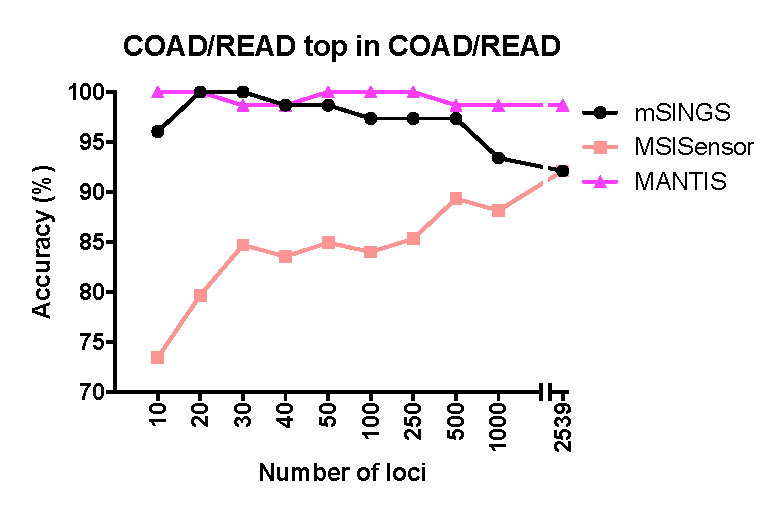
\includegraphics[width=\linewidth,keepaspectratio]{images/msilandscape/tool_performance_coadread_loci_coadread}
		\caption{}\label{fig:msilandscape:tool_performance_coadread_loci_coadread}
	\end{subfigure}%
	\hfill%
	\begin{subfigure}{0.33\textwidth}
		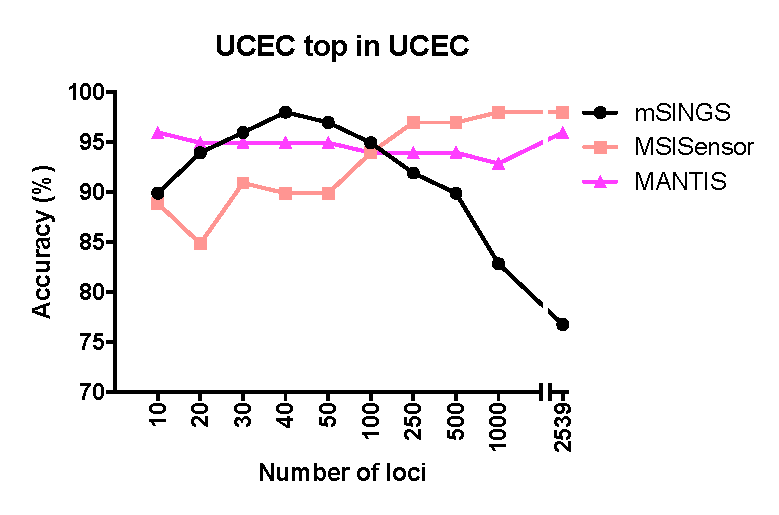
\includegraphics[width=\linewidth,keepaspectratio]{images/msilandscape/tool_performance_ucec_loci_ucec}
		\caption{}\label{fig:msilandscape:tool_performance_ucec_loci_ucec}
	\end{subfigure}%
	\hfill%
	\begin{subfigure}{0.33\textwidth}
		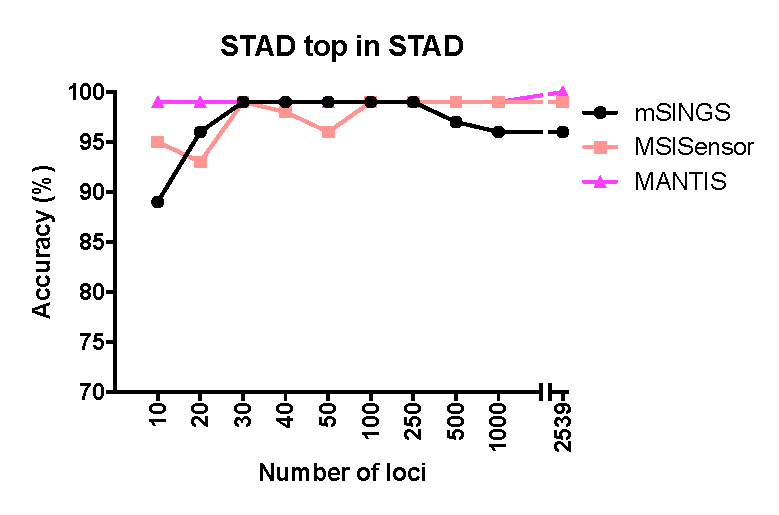
\includegraphics[width=\linewidth,keepaspectratio]{images/msilandscape/tool_performance_stad_loci_stad}
		\caption{}\label{fig:msilandscape:tool_performance_stad_loci_stad}
	\end{subfigure}
	\par
	\begin{subfigure}{0.33\textwidth}
		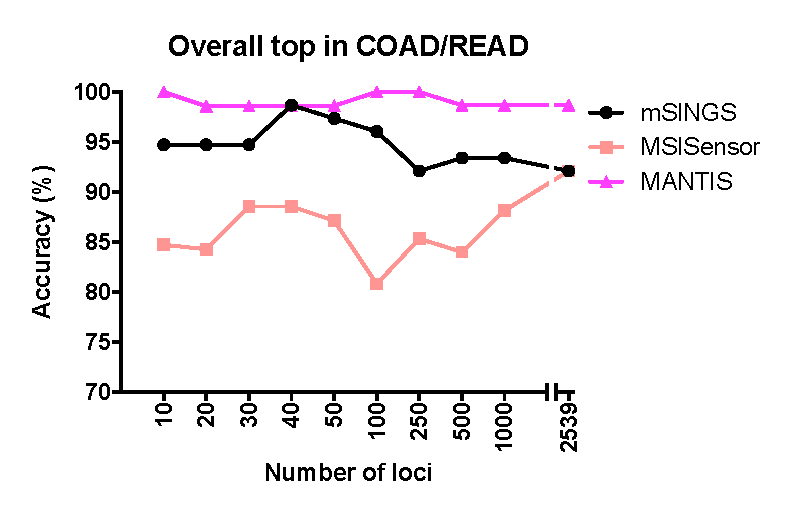
\includegraphics[width=\linewidth,keepaspectratio]{images/msilandscape/tool_performance_top_loci_coadread}
		\caption{}\label{fig:msilandscape:tool_performance_top_loci_coadread}
	\end{subfigure}%
	\hfill%
	\begin{subfigure}{0.33\textwidth}
		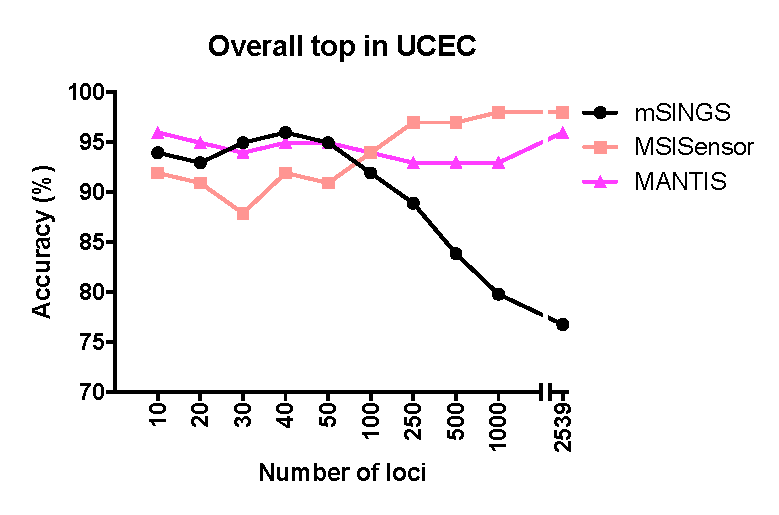
\includegraphics[width=\linewidth,keepaspectratio]{images/msilandscape/tool_performance_top_loci_ucec}
		\caption{}\label{fig:msilandscape:tool_performance_top_loci_ucec}
	\end{subfigure}%
	\hfill%
	\begin{subfigure}{0.33\textwidth}
		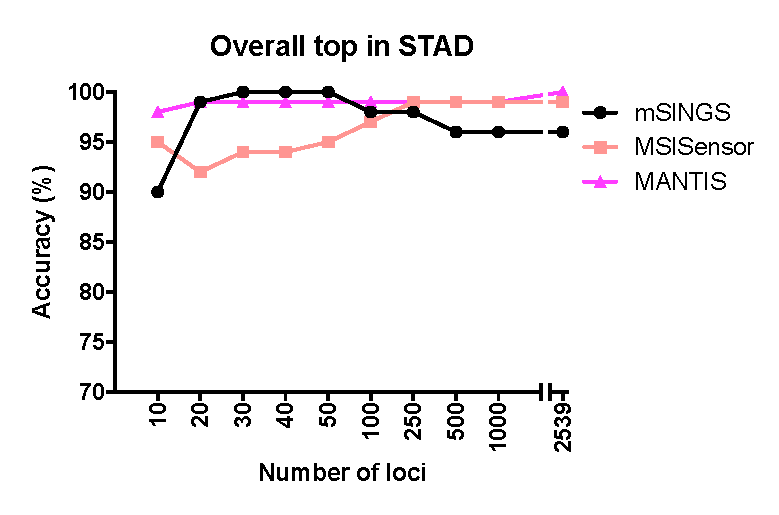
\includegraphics[width=\linewidth,keepaspectratio]{images/msilandscape/tool_performance_top_loci_stad}
		\caption{}\label{fig:msilandscape:tool_performance_top_loci_stad}
	\end{subfigure}
	\par
	\begin{subfigure}{0.33\textwidth}
		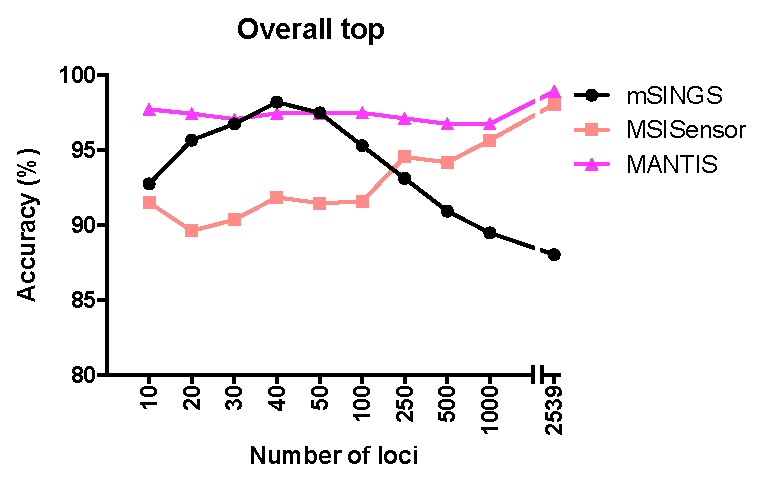
\includegraphics[width=\linewidth,keepaspectratio]{images/msilandscape/tool_performance_top_loci_all}
		\caption{}\label{fig:msilandscape:tool_performance_top_loci_all}
	\end{subfigure}
	\caption[Performance of mSINGS, MSISensor and MANTIS with their respective top-performing loci.]{The performance of mSINGS, MSISensor and MANTIS with their respective top-performing loci. For each tool, and within the COAD/READ, UCEC and STAD samples, the top-performing loci were determined, and the performance of each tool with these loci in each COAD/READ (\subref{fig:msilandscape:tool_performance_coadread_loci_coadread}), UCEC (\subref{fig:msilandscape:tool_performance_ucec_loci_ucec}) and STAD (\subref{fig:msilandscape:tool_performance_stad_loci_stad}) cohorts was evaluated with top tool- and cohort-specific loci (10-1000). In addition, the top-performing loci across all cohorts combined were determined, and performance of each tool with varying numbers of all-cohort top-performing loci in the COAD/READ (\subref{fig:msilandscape:tool_performance_top_loci_coadread}), UCEC (\subref{fig:msilandscape:tool_performance_top_loci_ucec}) and STAD (\subref{fig:msilandscape:tool_performance_top_loci_stad}) cohorts was determined. This analysis was also performed for all cohorts combined (\subref{fig:msilandscape:tool_performance_top_loci_all}). The results with 2,539 loci (without loci shortlisting) are included for reference.}
	\label{fig:msilandscape:tool_performance_top_loci}
\end{figure}

Previous studies have suggested that different MSI positive cancers may have specific microsatellite loci that are most commonly unstable \cite{faulkner2004,hempelmann2015}. For each MSI analysis tool, we sought to account for this by identifying the top-performing loci in each cancer type separately. Unlike in the analysis above, the 10, 20, 30, 40, 50, 100, 250, 500 and 1000 best-performing loci for each tool were determined for each COAD/READ, UCEC and STAD cohort separately (Supplemental File~S\thechapter{}.7). Each tool was then run over each cancer type, with respective top tool-specific and cancer-specific loci (Figure~\ref{fig:msilandscape:tool_performance_top_loci}a--c). Trends described in the previous analysis remained the same, with performance slightly higher throughout. However in UCEC at 40 loci, mSINGS performed better than MSISensor and MANTIS (98.0\% accuracy, vs.\ 89.9\% and 94.9\% respectively). Also, MANTIS and mSINGS both performed notably better (98.7\%) than MSISensor (83.6\%) when evaluating COAD/READ samples with 40 loci. The experiments show that the choice of loci being evaluated plays a part in tool performance. While an optimized target panel may allow all tools to perform well, MANTIS exhibits the most stable performance even without such optimizations, providing accurate performance using existing whole exome data.

\subsection{MSI landscape}
\label{ssec:msilandscape:landscape_results}
\begin{figure}[htp]
    \centering
    \begin{subfigure}{0.95\textwidth}
        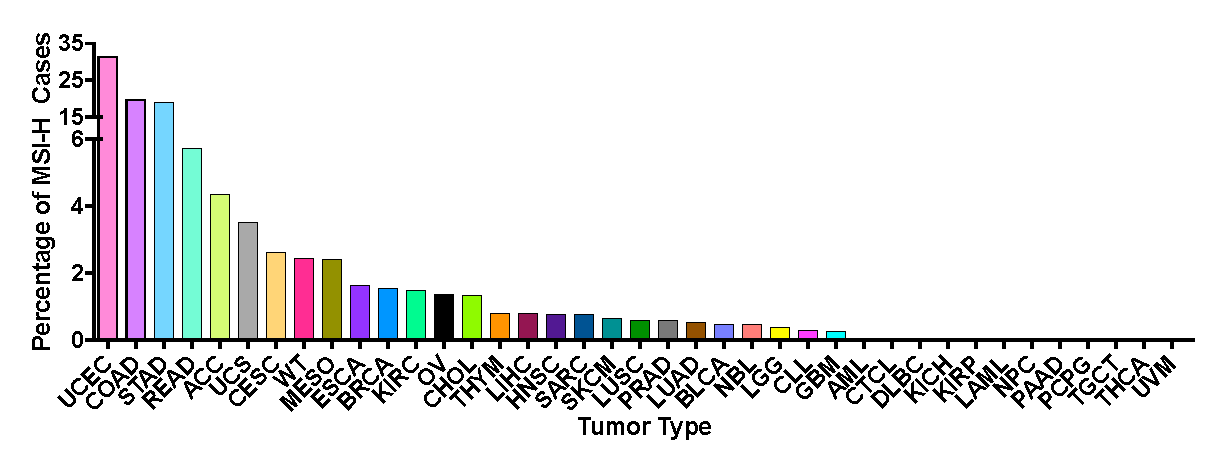
\includegraphics[width=\linewidth,keepaspectratio]{images/msilandscape/msi_landscape_bars}
        \caption{}\label{fig:msilandscape:msi_landscape_bars}
    \end{subfigure}
    
    \begin{subfigure}{0.95\textwidth}
        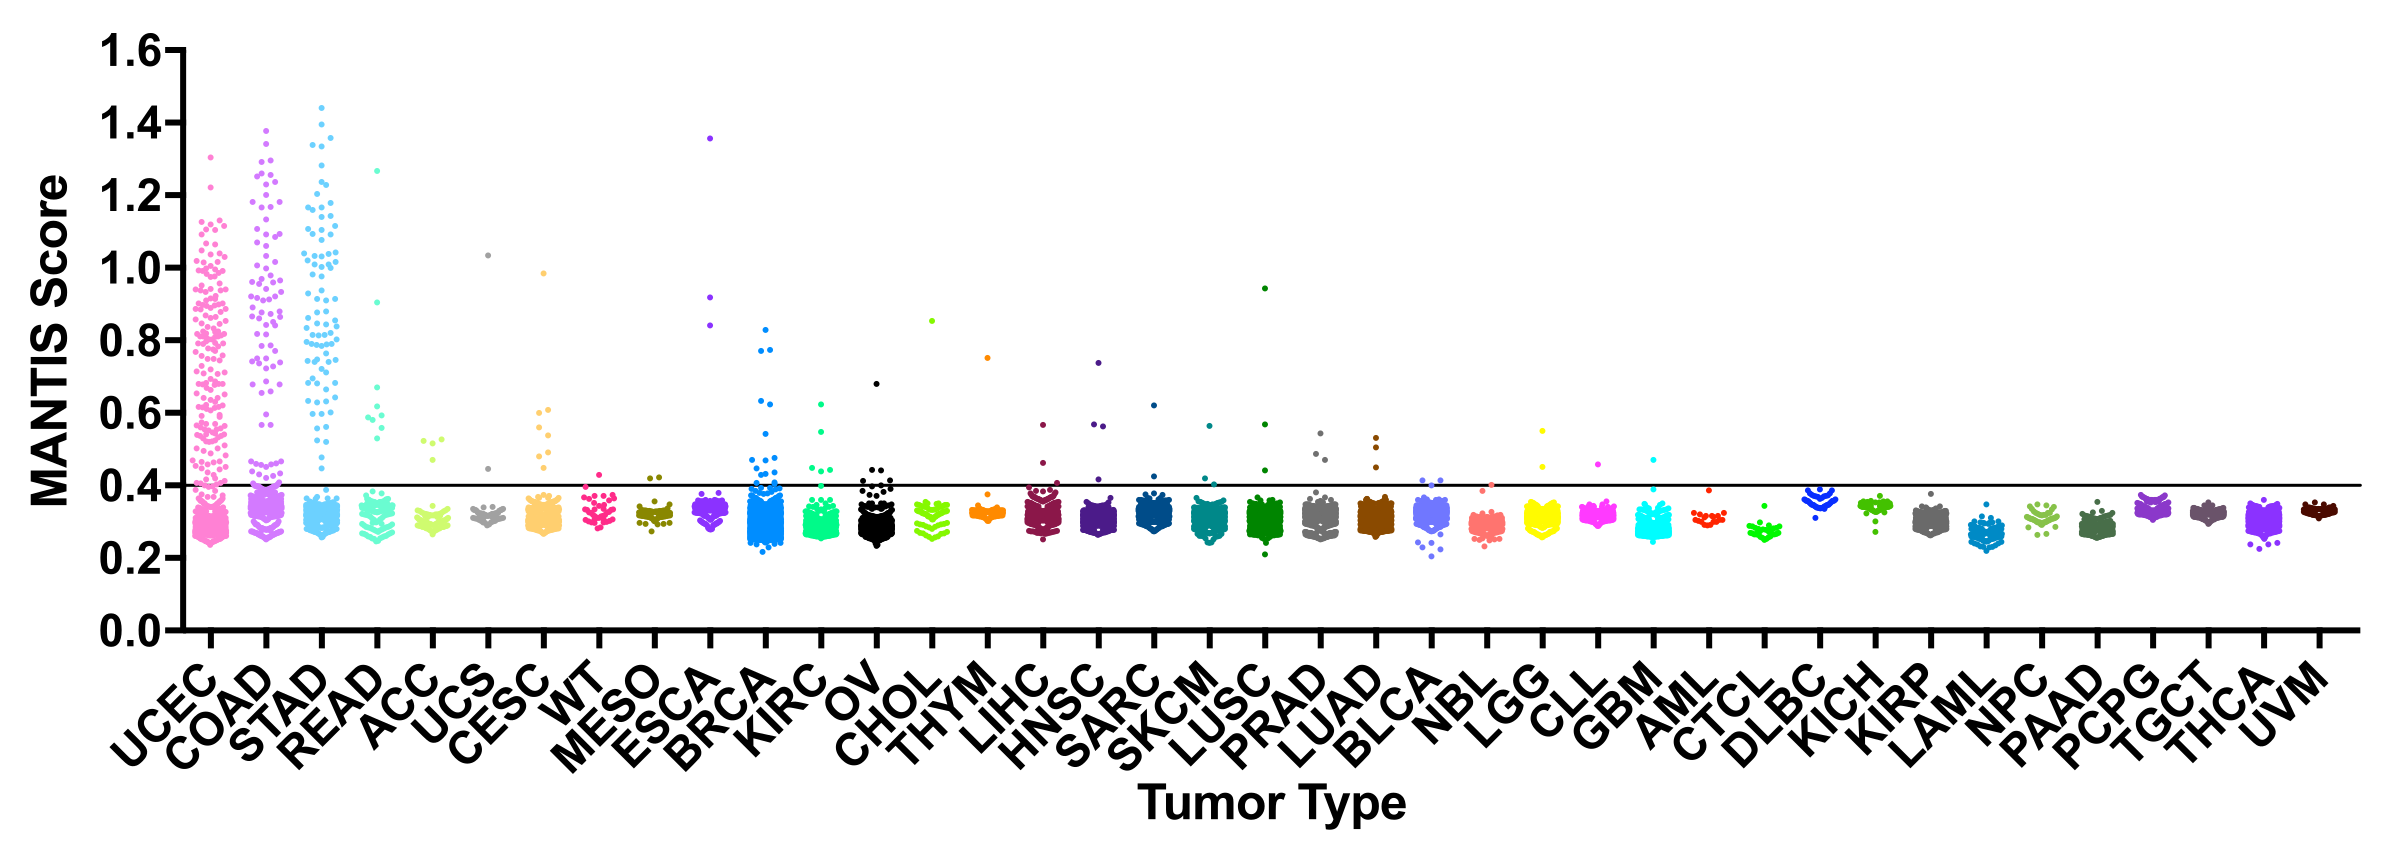
\includegraphics[width=\linewidth,keepaspectratio]{images/msilandscape/msi_landscape_dist}
        \caption{}\label{fig:msilandscape:msi_landscape_dist}
    \end{subfigure}
    \caption[Prevalence of MSI across 39 human cancer types.]{Prevalence of microsatellite instability (MSI) across 39 human cancer types. (\subref{fig:msilandscape:msi_landscape_bars}) MSI prevalence was detected across 39 tumor types. The total number of tumors and the percentage of cases called MSI-H in each cohort is listed in Table~\ref{table:msilandscape:landscape_summary}. (\subref{fig:msilandscape:msi_landscape_dist}) The relative level of instability, as measured by MANTIS score, is shown across all 39 tumor types. Note that for chronic lymphocytic leukemia (CLL), the listed MSI prevalence in panel (\subref{fig:msilandscape:msi_landscape_bars}) is out of 279 patients, and all 338 tumors are shown in panel (\subref{fig:msilandscape:msi_landscape_dist}), as some patients in this cohort had multiple tumors. MANTIS threshold cutoff of 0.4 is depicted with a dashed line. Cancer type abbreviations are listed in Appendix~\ref{app.cancerabbrev}.}
    \label{fig:msilandscape:msi_landscape}
\end{figure}
We analyzed paired whole exome sequencing data from 11,139 tumor-normal samples; 10,415 from the TCGA \cite{tcgageneric} database, 280 from the TARGET \cite{target} database, and 444 from other studies \cite{landau2015,choi2015,zheng2016,ong2012,chanon2013}, representing 39 distinct cancer types. MSI was detected in 27 of these 39 cancer types (Figure~\ref{fig:msilandscape:msi_landscape_bars}, Table~\ref{table:msilandscape:landscape_summary}, Supplemental File~S\thechapter{}.5). The disease-specific prevalence of MSI varied widely, from 31.4\% in endometrial carcinoma to 0.25\% in glioblastoma multiforme. MSI was not detected in 12 cancer types (Figure~\ref{fig:msilandscape:msi_landscape}). Of the 27 cancer types with MSI, 12 were found to have more than a single MSI-H tumor present, and MSI-H prevalence greater than 1\%. The relative level of instability, as measured by MANTIS score, varied substantially among cancer types that were MSI-H (Figure~\ref{fig:msilandscape:msi_landscape_dist}). In addition, we attempted to determine which specific microsatellite loci performed best across the greatest number of cancer types (Supplemental File~S\thechapter{}.8). Out of 2,530 loci, we identified 22 loci that, within at least five cohorts, had a MSI-H versus MSS difference score greater than 0.75 and were sufficiently covered by at least 50\% of samples in the cohort (Table~\ref{table:msilandscape:top_loci_landscape}). Only two loci assessed in the Bethesda \cite{boland1998} and Promega\textsuperscript\texttrademark{} \cite{bacher2004} MSI-PCR panels were included in our 2,530 loci, and neither of these were within the set of 22 top-performing loci. These results indicate a striking heterogeneity of microsatellite instability patterns across various cancer types.

\begin{figure}[ht]
    \centering
	\begin{subfigure}{0.33\textwidth}
		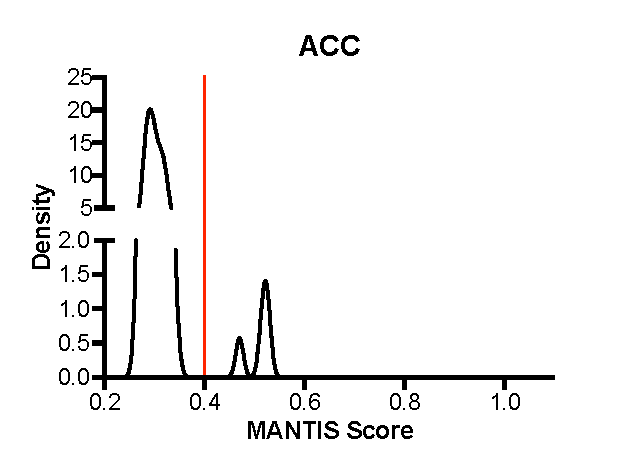
\includegraphics[width=\linewidth,keepaspectratio]{images/msilandscape/landscape_kd_acc}
		\caption{}\label{fig:msilandscape:landscape_kd_acc}
	\end{subfigure}%
	\hfill%
	\begin{subfigure}{0.33\textwidth}
		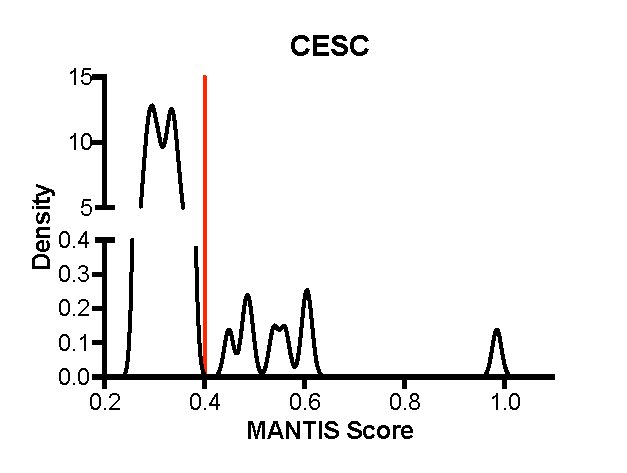
\includegraphics[width=\linewidth,keepaspectratio]{images/msilandscape/landscape_kd_cesc}
		\caption{}\label{fig:msilandscape:landscape_kd_cesc}
	\end{subfigure}%
	\hfill%
	\begin{subfigure}{0.33\textwidth}
		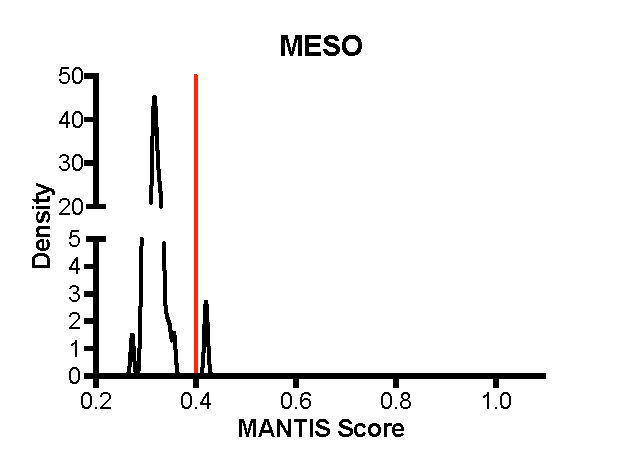
\includegraphics[width=\linewidth,keepaspectratio]{images/msilandscape/landscape_kd_meso}
		\caption{}\label{fig:msilandscape:landscape_kd_meso}
	\end{subfigure}
	\caption[Kernel density plots of MANTIS scores within ACC, CESC, and MESO.]{Kernel density plots of MANTIS scores within (\subref{fig:msilandscape:landscape_kd_acc}) adrenocortical carcinoma (ACC), (\subref{fig:msilandscape:landscape_kd_cesc}) cervical squamous cell carcinoma and endocervical adenocarcinoma (CESC), and (\subref{fig:msilandscape:landscape_kd_meso}) mesothelioma (MESO)\@. The dotted line denotes the average distance threshold of 0.4, used by MANTIS to differentiate microsatellite instability high from microsatellite stable tumors. ACC: $n = 92$, kernel bandwidth ($h$) $= 7.6 \times 10^{-3}$; CESC: $n = 305$, $h = 9.4 \times 10^{-3}$; MESO: $n = 83$, $h = 3.2 \times 10^{-3}$.}
	\label{fig:msilandscape:landscape_kd_acc_cesc_meso}
\end{figure}
All four disease types with the highest rates of MSI prevalence were Lynch syndrome-associated tumor types previously known to exhibit MSI: endometrial carcinoma, colon adenocarcinoma, gastric adenocarcinoma, and rectal adenocarcinoma. Consistent with previous studies, MSI was found to be more frequent in colon (19.7\%) than rectal (5.7\%) adenocarcinoma \cite{hause2016,phipps2013}. Of importance, MSI was detected in three cancer types that have not been previously well characterized, most notably adrenocortical carcinoma (ACC, 4.3\%), cervical squamous cell carcinoma and endocervical adenocarcinoma (CESC, 2.6\%), and mesothelioma (MESO, 2.4\%) (Figure~\ref{fig:msilandscape:msi_landscape_bars}). To further investigate MSI status classifications, kernel density estimation \cite{parzen1962,davis2011} was performed on the MANTIS scores for these tumor types. This indicated clear distinctions between samples MANTIS called MSI-H from samples called MSS (Figure~\ref{fig:msilandscape:landscape_kd_acc_cesc_meso}). Kernel density estimation was also performed on all other tumor types tested (Figure~\ref{fig:msilandscape:landscape_kd_others}).

\begin{figure}[htp]
    \centering
    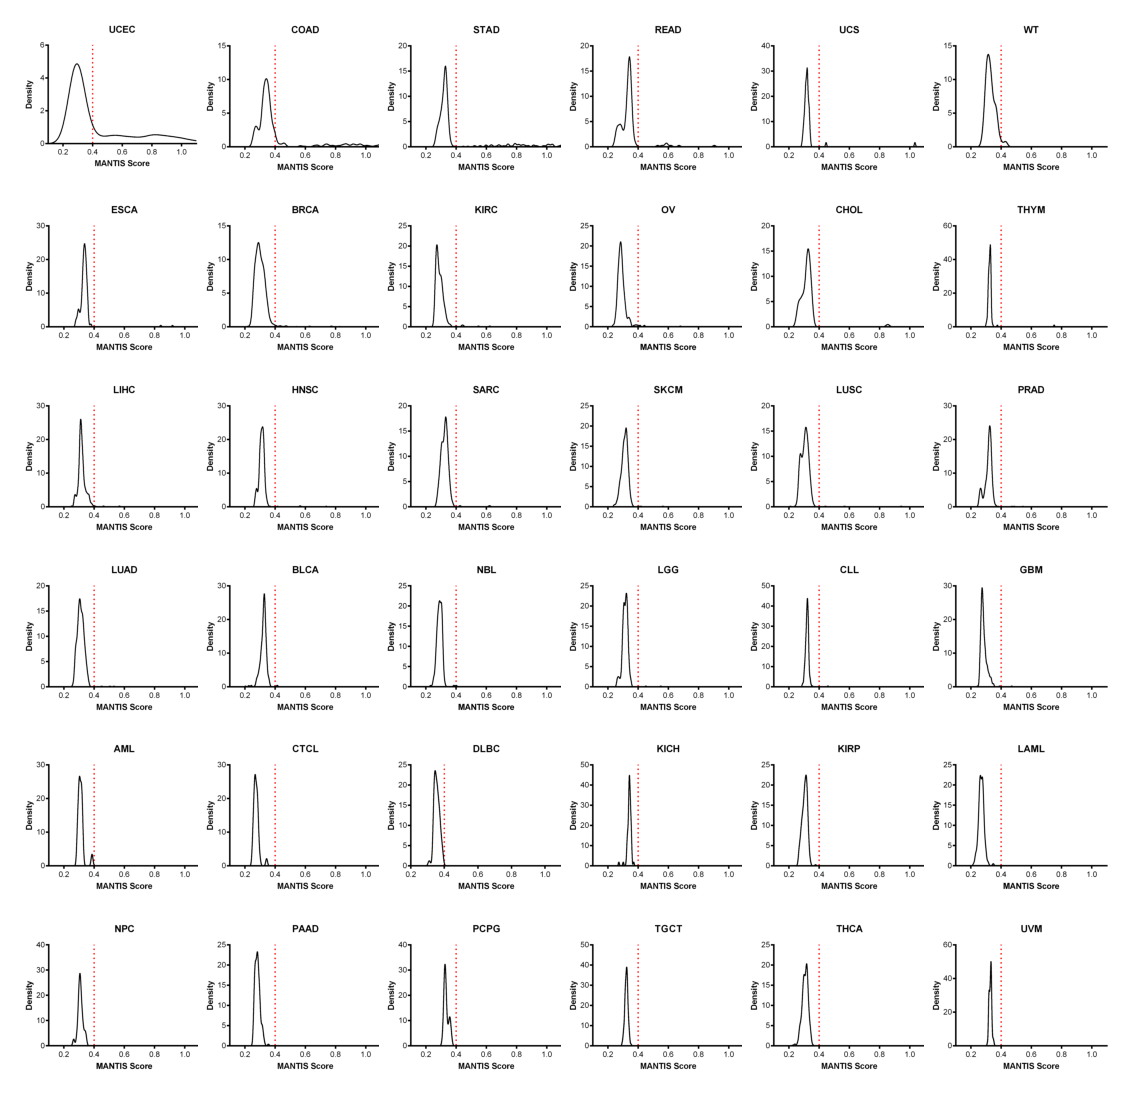
\includegraphics[width=0.98\linewidth,keepaspectratio]{images/msilandscape/landscape_kd_others}
    \caption[Kernel density plots of MANTIS scores within 36 cancer types.]{Kernel density plots of MANTIS scores within 36 cancer types. The dotted line denotes the average distance threshold of 0.4, used by MANTIS to differentiate microsatellite instability high from microsatellite stable tumors. UCEC: kernel bandwidth ($h$) = $4.89 \times 10^{-2}$. COAD: $h = 1.13 \times 10^{-2}$. STAD: $h = 7.59 \times 10^{-3}$. READ: $h = 9.16 \times 10^{-3}$. UCS: $h = 4.10 \times 10^{-3}$. WT: $h = 1.27 \times 10^{-2}$. ESCA: $h = 5.02 \times 10^{-3}$. BRCA: $h = 7.41 \times 10^{-3}$. KIRC: $h = 6.83 \times 10^{-3}$. OV: $h = 5.23 \times 10^{-3}$. CHOL: $h = 1.17 \times 10^{-2}$. THYM: $h = 3.08 \times 10^{-3}$. LIHC: $h = 4.42 \times 10^{-3}$. HNSC: $h = 4.25 \times 10^{-3}$. SARC: $h = 7.14 \times 10^{-3}$. SKCM: $h = 5.32 \times 10^{-3}$. LUSC: $h = 7.13 \times 10^{-3}$. PRAD: $h = 5.31 \times 10^{-3}$. BLCA: $h = 4.40 \times 10^{-3}$. CLL: $h = 2.64 \times 10^{-3}$. GBM: $h = 4.38 \times 10^{-3}$. AML: $h = 6.13 \times 10^{-3}$. CTCL: $h = 5.86 \times 10^{-3}$. DLBC: $h = 6.68 \times 10^{-3}$. KICH: $h = 3.34 \times 10^{-3}$. KIRP: $h = 5.16 \times 10^{-3}$. LAML: $h = 5.28 \times 10^{-3}$. NPC: $h = 6.09 \times 10^{-3}$. PAAD: $h = 5.36 \times 10^{-3}$. PCPG: $h = 5.04 \times 10^{-3}$. TGCT: $h = 3.40 \times 10^{-3}$. THCA: $h = 5.09 \times 10^{-3}$. UVM: $h = 3.06 \times 10^{-3}$.}
    \label{fig:msilandscape:landscape_kd_others}
\end{figure}

\subsection{Comparing TMB and signatures between MSI-H and MSS tumors}
\begin{figure}[ht]
    \centering
    \hfill%
	\begin{subfigure}{0.25\textwidth}
		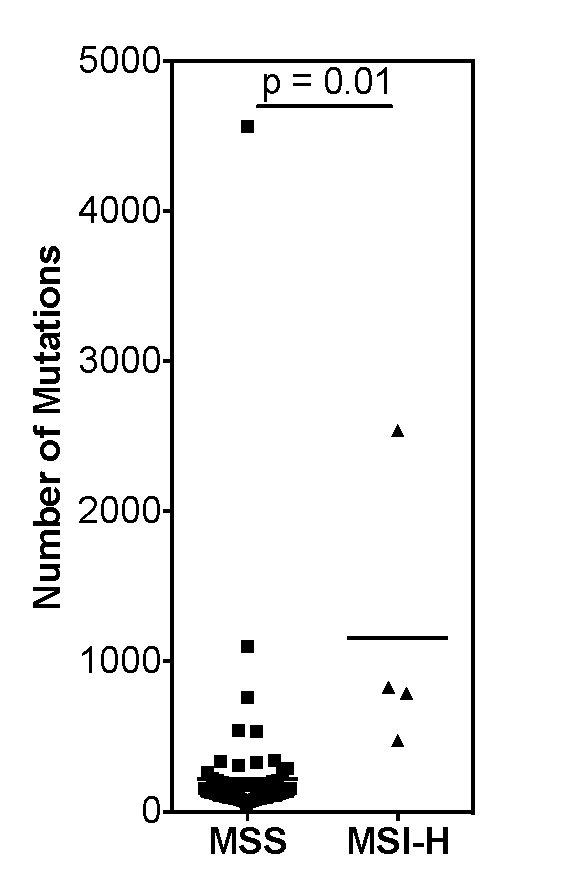
\includegraphics[width=\linewidth,keepaspectratio]{images/msilandscape/tmb_acc}
		\caption{}\label{fig:msilandscape:tmb_acc}
	\end{subfigure}%
	\hfill%
	\begin{subfigure}{0.25\textwidth}
		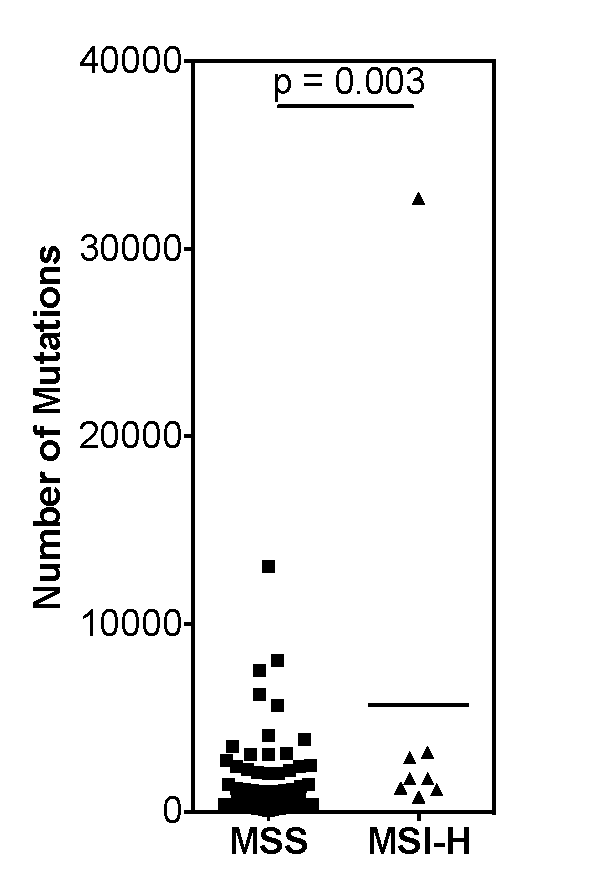
\includegraphics[width=\linewidth,keepaspectratio]{images/msilandscape/tmb_cesc}
		\caption{}\label{fig:msilandscape:tmb_cesc}
	\end{subfigure}%
	\hfill%
	\begin{subfigure}{0.25\textwidth}
		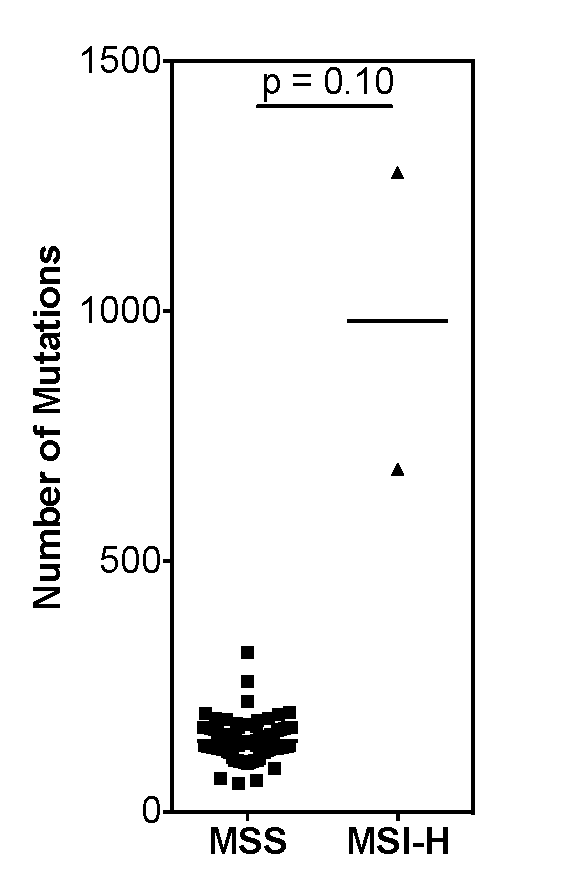
\includegraphics[width=\linewidth,keepaspectratio]{images/msilandscape/tmb_meso}
		\caption{}\label{fig:msilandscape:tmb_meso}
	\end{subfigure}%
	\hfill
	\caption[TMB correlates with MSI-H within ACC and CESC.]{Tumor mutational burden correlates with microsatellite instability high (MSI-H) status within adrenocortical carcinoma (ACC) and cervical squamous cell carcinoma and endocervical adenocarcinoma (CESC)\@. Mutational burden is listed for (\subref{fig:msilandscape:tmb_acc}) ACC, (\subref{fig:msilandscape:tmb_cesc}) CESC, and (\subref{fig:msilandscape:tmb_meso}) mesothelioma (MESO)\@. $P$ values were calculated using the Welch two-sample $t$-test of log-normalized absolute somatic mutation counts. Variant calling was performed by using MuTect (Section~\ref{ssec:msilandscape:variant_calling}), and all passing variants were included (nonsynonymous or synonymous).}
	\label{fig:msilandscape:tmb_acc_cesc_meso}
\end{figure}
Since Lynch syndrome-associated MSI-H tumors have been shown to have higher somatic tumor mutation burden (TMB) \cite{le2015,gatalica2016}, we performed further analysis to detect potential hypermutation in MSI-H ACC, CESC and MESO\@. Somatic variant calling was performed on whole exome samples from these four cancer types, and the mean absolute number of somatic mutations (both nonsynonymous and synonymous) was found to be increased among MSI-H versus MSS tumors within their own cohorts (Figure~\ref{fig:msilandscape:tmb_acc_cesc_meso}). In particular, an average of 1,157 somatic mutations were detected within MSI-H ACC samples, versus 216 within MSS ACC ($p = 0.01$). An average of 5,675 somatic mutations were detected within MSI-H CESC samples, versus 639 within MSS CESC ($p = 0.003$). Although statistical significance was not reached within MESO, MSI-H MESO tumors had, on average, nearly a seven-fold increase in TMB when compared to MSS MESO tumors (982 versus 142, $p = 0.10$). All $p$ values were calculated using Welch's two-sample $t$-test with log normalization. These results indicate that microsatellite instability in ACC and CESC is correlated with high TMB\@.

\begin{figure}[htp]
    \centering
    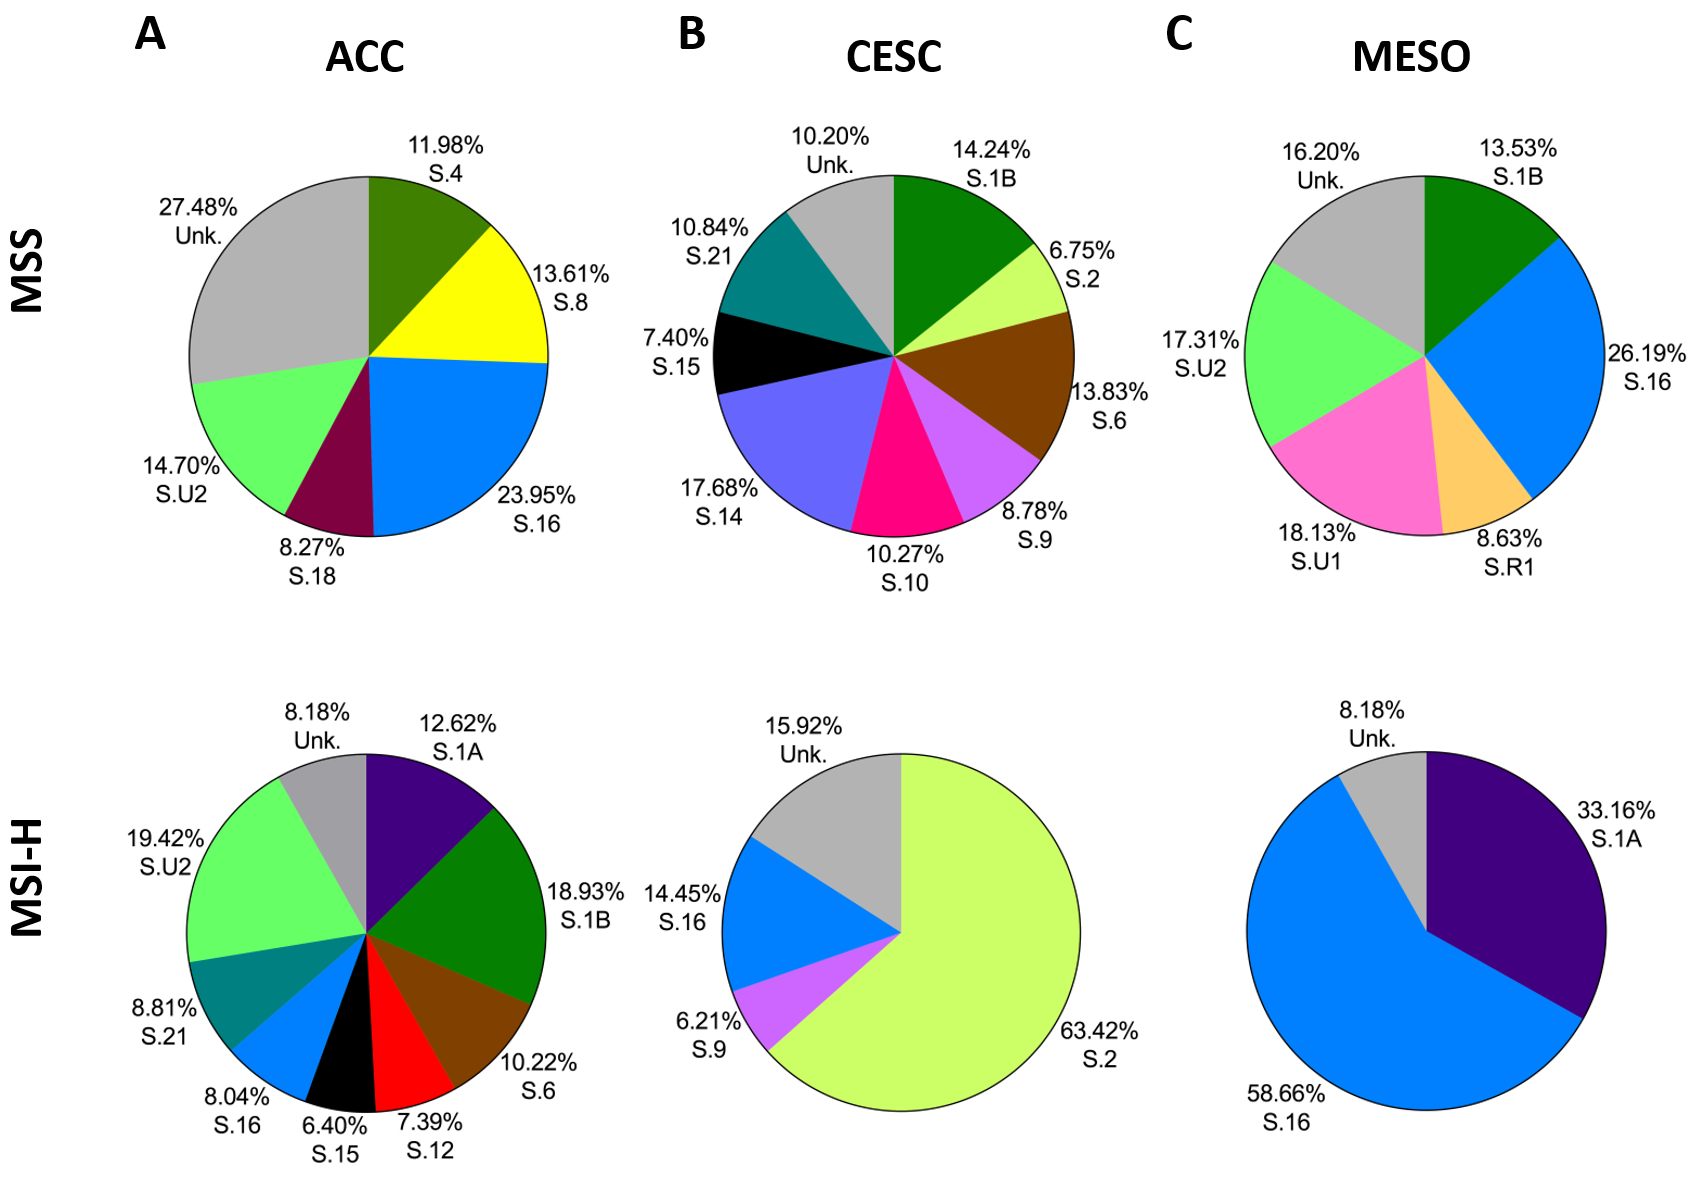
\includegraphics[width=0.98\linewidth,keepaspectratio]{images/msilandscape/sigs_acc_cesc_meso}
    \caption[Patterns of mutational signatures across cancers by microsatellite instability status.]{Patterns of mutational signatures (S) across cancers by microsatellite instability status. Cancers: (\textbf{A}) adrenocortical carcinoma (ACC), (\textbf{B}) cervical squamous cell carcinoma and endocervical adenocarcinoma (CESC), and (\textbf{C}) mesothelioma (MESO)\@. Mutational signatures were called using deconstructSigs from pooled variants from all MSI-H or MSS tumors within each cohort within ACC, CESC, and MESO\@. Unk., unknown.}
    \label{fig:msilandscape:sigs_acc_cesc_meso}
\end{figure}
To further investigate the observed somatic mutations in MSI-H versus MSS ACC, CESC, and MESO tumors, mutational signature analysis was performed using a set of 27 signatures introduced by Alexandrov \textit{et al} \cite{alexandrov2013}. A mutational signature defines a pattern of preferential somatic mutation types, and may be associated with a known biological process or cancer type. This analysis was first performed on pooled mutations among MSI-H or MSS samples within each of these three cancer cohorts (Figure~\ref{fig:msilandscape:sigs_acc_cesc_meso}). No clear pattern of signature differences was evident from this pooled analysis. Next, mutational signature analysis was performed for each individual case within these cohorts without pooling (Supplemental File~S\thechapter{}.9). Differences among signature prevalence in ACC, CESC, and MESO did not reach statistical significance. $P$ values were calculated using the two-sided Fisher exact test (using signature presence or absence), with Benjamini correction for multiple hypotheses.

\subsection{MMR pathway alterations}
\begin{table}[htbp]
    \centering
    {\small
    \begin{tabular}{lc:cccccc:c}
        & \textbf{Sample} & & & & & & \\
        \textbf{Variable} & \textbf{Count} & \textbf{\textit{MSH2}} & \textbf{\textit{MSH6}} & \textbf{\textit{MLH1}} & \textbf{\textit{PMS2}} & \textbf{\textit{EXO1}} & \textbf{\textit{POLE}} & \textbf{Any} \\
        \hline
        ACC & & & & & & & & \\
        \hphantom{---} MSS   & 88 & 1 & 1 & 0 & 1 & 0 & 1 & 4 \\
        \hphantom{---} MSI-H & 4 & 0 & 0 & 1 & 0 & 0 & 1 & 2 \\
        \hline
        CESC & & & & & & & & \\
        \hphantom{---} MSS   & 297 & 3 & 3 & 5 & 0 & 3 & 10 & 22 \\
        \hphantom{---} MSI-H & 8 & 0 & 1 & 3 & 1 & 1 & 2 & 6 \\
        \hline
        MESO & & & & & & & & \\
        \hphantom{---} MSS   & 81 & 0 & 1 & 0 & 0 & 0 & 1 & 2 \\
        \hphantom{---} MSI-H & 2 & 1 & 0 & 0 & 0 & 0 & 1 & 1 \\
        \hline
        ACC + CESC & & & & & & & & \\
        \hphantom{ACC }+ MESO & & & & & & & & \\
        \hphantom{---} MSS   & 466 & 4 & 5 & 5 & 1 & 3 & 12 & 28 \\
        \hphantom{---} MSI-H & 14 & 1 & 1 & 4 & 1 & 1 & 3 & 9
    \end{tabular}}
    \caption[Frequency of predicted deleterious MMR mutations in ACC, CESC, and MESO.]{Frequency of predicted deleterious MMR mutations in ACC, CESC, and MESO\@. Listed are the number of samples (MSS or MSI-H) with at least one predicted deleterious mutation in \textit{MSH2}, \textit{MSH6}, \textit{MLH1}, \textit{PMS2}, \textit{EXO1}, \textit{POLD1}, \textit{POLE}, or any of these genes (Any). Mutations were called using MuTect (Section~\ref{ssec:msilandscape:variant_calling}) and included in this table if the DANN pathogenicity score was $>0.96$.}
    \label{table:msilandscape:mmr_muts}
\end{table}
MSI-H Lynch syndrome-associated tumors are known to lack expression or function of at least one MMR protein. Therefore, we analyzed somatic mutations predicted to be deleterious (by DANN) in the mismatch repair genes \textit{MSH2}, \textit{MSH6}, \textit{MLH1}, \textit{PMS2} and \textit{EXO1}, and the proofreading DNA polymerases \textit{POLD1} and \textit{POLE}, among MSI-H and MSS samples within ACC, CESC, and MESO (Table~\ref{table:msilandscape:mmr_muts}), Supplemental File~S\thechapter{}.10). Though POLD1 and POLE are not considered MMR proteins, mutations in these genes have been shown to lead to somatic hypermutation \cite{tcgacoadread,johnson2015}. 64\% of MSI-H cases and 7\% of MSS cases within these cohorts were found to contain at least one predicted deleterious somatic mutation in at least one of these genes. However, given that these samples were sequenced with potentially different exome captures, and the increased mutational burden of MSI-H tumors, we could not determine the statistical significance of this finding.

\section{Discussion}
We have developed a new tool, MANTIS, for detecting MSI status using paired tumor-normal sequencing data. Unlike other tools, MANTIS analyzes the instability of a normal-tumor sample pair as an aggregate of loci instead of individual loci differences. The approach allows the tool to evaluate the general instability present in a tumor sample, using the data from the corresponding normal sample as an error-correcting baseline. Furthermore, by pooling the scores of all the loci and treating the average as the instability score, the evaluation benefits from the law of large numbers by reducing the impact that sequencing errors or poorly performing loci may have on the results.

We also analyzed the performance of MANTIS, mSINGS, and MSISensor with samples from six cancer types. Overall, MANTIS demonstrated high accuracy across a range of cancer types, and in many cases with restricted sets of well-performing loci. Prior tools have previously been applied to only one of two cancer types, endometrial (MSISensor) and colorectal (mSINGS)\@. With their recommended thresholds, mSINGS and MSISensor are less robust across a range of loci numbers than MANTIS\@. This appears to be due to the inclusion of poorly performing loci with low sensitivity in the full set of 2,539 loci. mSINGS and MSISensor call loci unstable or stable, and MANTIS calculates the instability at each locus. Suboptimal loci may be missed entirely by mSINGS and MSISensor, but still have some increased instability in MSI-H vs.\ MSS samples. Niu \textit{et al} recommend a relatively low threshold of 3.5 for MSISensor (vs.\ 20\% used by mSINGS and MSI-PCR)\@. This seems to effectively compensate for these poorly performing loci with a large panel, but greatly reduces the specificity of MSISensor when these loci are removed, as in the lists of top-performing loci. Conversely, the threshold of 0.2 (20\%) used by mSINGS is effective with a smaller panel of well-performing loci such as the mSINGS authors' panel MSIplus \cite{hempelmann2015}, but this threshold limits the sensitivity of mSINGS with a larger panel (Table~\ref{table:msilandscape:tool_accuracy}).

Results from UCEC were least concordant with the above trends. With the full set of 2,539 loci, MSISensor performed best, followed closely by MANTIS and distantly by mSINGS\@. This may potentially arise from differences in the microsatellite instability signatures between COAD/READ and UCEC, the existence of which is supported by previous findings \cite{alhopuro2012,kim2013}. A recent overview of microsatellite instability across multiple cancer types by Hause \textit{et al} further found significant variance in the number of unstable loci present between samples from different diseases \cite{hause2016}. Another potential explanation is that, because mSINGS was developed only with COAD/READ data and MSISensor only with UCEC data, these tools may be overfit to those cancer types. MANTIS, in contrast, was developed and tested using data from multiple cancer types, alleviating the potential overfitting issues that may occur when only including data from a single disease.

Like any NGS-based method, MANTIS performance depends on read coverage, a limitation not shared by MSI-PCR and IHC\@. Most current clinical guidelines for management of MSI positive tumors are based on a percentage of unstable loci. Current approaches for MSI detection (such as mSINGS, MSISensor, and MSI-PCR) use a discrete fraction of unstable loci to determine to make calls on the status of a sample, but MANTIS provides a continuously valued MSI score that may provide greater utility in determining the level of MSI present in a tumor. Findings by Hause \textit{et al} give further credence to this hypothesis, indicating that microsatellite instability may best be viewed as a scaled genotype rather than a simple binary positive or negative classification \cite{hause2016}.

We chose MANTIS, mSINGS, and MSISensor for this study since these three tools use NGS to directly assess microsatellite loci in DNA\@. Other NGS-based methods have been described that indirectly assess MSI through analysis of somatic mutations. MSIseq \cite{nihuang2015} employs machine learning classification techniques to correlate indels throughout repeat regions to MSI status. Stadler \textit{et al} \cite{stadler2016} describe a method utilizing a custom NGS assay, and correlating somatic missense and nonsense mutations in protein-coding regions with MSI status. Additionally, Lu \textit{et al} \cite{lu2013} describe an algorithm for determining MSI status from RNA-seq data. MSIseq was not included in this study as it is a classifier that only reports MSI-H vs.\ non-MSI-H, without a score or percentage, or information about the instability of particular loci. The Stadler \textit{et al} and Lu \textit{et al} methods were not included since they cannot be run with the same whole exome sequencing input data, requiring a custom deep-sequenced panel and RNA-seq data, respectively.

Currently, MMR and MSI status are determined in the clinical setting with IHC and MSI-PCR\@. Conventional multiplex MSI-PCR testing is reported to have 97\% sensitivity and 95\% specificity. IHC is reported to have 92.4\% sensitivity and 99.6\% specificity \cite{zhang2013}. MSI-PCR with the standard five Bethesda loci is well described for COAD/READ and UCEC \cite{armaghany2012}, but has been shown to perform less accurately in other diseases such as acute myeloid leukemia \cite{faulkner2004}, and may miss MSI in other tumor types. Consideration of only five loci renders conventional MSI-PCR highly susceptible to errors in processing or interpretation of any one locus, and adding additional loci increases cost. IHC is able to effectively determine the presence or absence of the mismatch repair proteins targeted. Unfortunately, IHC cannot detect loss-of-function mutations that do not affect the antigenicity of targeted proteins, or changes to MMR proteins not targeted \cite{shia2015}. Additionally, MSI-PCR and IHC require human interpretation, unlike computational NGS-based methods. Lastly, both MSI-PCR and IHC are clinical laboratory tests that consume fractions of patient tumor samples, unlike computational methods that could be multiplexed with other NGS assays for detecting somatic mutations.

As a tumor vs.\ normal algorithm, MANTIS avoids a time-consuming baseline generation step, eliminates potential baseline bias and allows processing of samples from different sequencing pipelines or tumor types without requiring a different baseline for each. Indeed, sequencing center bias may explain the discordance with mSINGS results from the 4 COAD/READ pairs sequenced at both BCM and BI (Table~\ref{table:msilandscape:coadread_by_site}). However, matched normal DNA is not always feasibly available for clinical laboratories that only sequence tumor samples, thus a tumor-only method such as mSINGS could reduce both sequencing time and cost to the patient.

The results of this study support several potential directions for future investigation. The accuracy of MANTIS with small numbers of loci suggests that MANTIS could be useful with a targeted sequencing panel designed for MSI testing in the clinic. With further investigation, incorporating MANTIS into clinical NGS pipelines may permit MSI testing on a large scale, and improve access to emerging therapies that exploit microsatellite instability in cancer. We have shown that MANTIS performs well in six cancer types; however it (along with other MSI tools) should be further evaluated in a wider variety of cancers. Of particular interest would be evaluation of MANTIS in neurologic, hematologic, pediatric and other malignancies, in which the landscape of MSI is considerably less well described than with COAD/READ and UCEC\@.

In this study, we have performed the largest-scale analysis of microsatellite instability in human cancer exomes as of July 2017, including 11,139 whole exome tumor-normal pairs from 39 cancer types. Compared to a study by Hause \textit{et al} \cite{hause2016}, we observed similar rates of MSI in 18 cancer types, and we further analyzed another 5,209 whole exome tumor-normal pairs from 21 additional cancer types. Additionally, we observed that MSI-H ACC and CESC tumors are significantly hypermutated, compared to MSS ACC and CESC tumors. We identified three cohorts with significant MSI prevalence that has not been previously well described. Of particular interest, we identified MSI in 4 of 92 (4.4\%) adrenocortical carcinoma cases. Previous studies of MSI in ACC have implicated Lynch syndrome as a risk factor for familial ACC \cite{challis2016,raymond2013} However, to our knowledge, NGS-based MSI analysis has not yet been applied to ACC\@.

MSI-H colorectal tumors have been previously shown to be exceptionally sensitive to therapy with PD-1 immune checkpoint inhibitors \cite{le2015}. Identification of MSI in novel tumor types may lead to an expanded role for immunotherapy, as well as a broader scope of clinical MSI testing \cite{dudley2016}. In addition, MSI is known to be prognostic within colorectal cancer \cite{kawakami2015}, which may apply in other cancer types as well. For instance, Hause \textit{et al} provide evidence that increasing MSI positively correlates with survival time. Clinical trials of immune checkpoint inhibitors are beginning or underway in ACC \cite{NCT02673333}, CESC \cite{NCT02635360}, and MESO \cite{NCT02784171,NCT02991482,NCT02707666,NCT02399371}, and a previous study of dendritic cell immunotherapy in ACC \cite{papewalis2006} demonstrated tumor marker but not clinical response. These studies may benefit from retrospective evaluation of MSI-H as a biomarker. Prospective expansion of clinical MSI testing to other cancer types may enlighten the prognostic and predictive value of MSI-H for non-colorectal cancers.

MMRd is well-recognized as the predominant cause of MSI within colorectal, endometrial and gastric cancers. Additionally, there have been anecdotal reports of ACC as a potential extracolonic manifestation of Lynch syndrome \cite{challis2016,raymond2013}. If future studies indicate that MSI in ACC, CESC, and/or MESO is indeed due to MMR deficiency, the findings of this study may implicate previously unappreciated cancer types as part of Lynch syndrome. Compared to germline alterations in MMR genes, somatic events are most often due to hypermethylation of CpG islands in the promoter region of \textit{MLH1} \cite{boland1998}. Further investigation is needed to elucidate other molecular mechanisms that can lead to MSI, as well as the downstream effects of MSI on tumor-specific biology. In addition, of the 9,569 tumors assessed in this study not within colorectal, endometrial, or gastric cancer, 77 (0.8\%) were MSI-H\@. Only 14 of these were within ACC, CESC, or MESO, compromising the statistical power of our mutational signature analysis. A larger cohort of MSI-H tumors would permit more comprehensive studies, including correlation with clinical data.

In summary, we have introduced a new MSI detection tool, MANTIS, and demonstrated its favorable performance compared to the previously published tools mSINGS and MSISensor. MANTIS exhibited the highest overall sensitivity and specificity within our test cohort comprising six cancer types, even with loci panels of varying size. Additionally, MANTIS also had the lowest resource consumption (\textless{}~1\% of the space and \textless{}~7\% of the memory required by mSINGS) and fastest running times (49.6\% and 8.7\% of the running times of MSISensor and mSINGS), respectively. We applied MANTIS to detect MSI in multiple additional cancer types including ACC, CESC, and MESO, indicating that MSI may affect non-Lynch syndrome tumor types. Within each cancer type having MSI, we identified which loci (among 2,530) were most predictive of overall tumor MSI status. With further analysis, these well-performing loci may form the basis of a targeted NGS panel for pan-cancer MSI detection. Additionally, we found that MSI-H tumors in ACC and CESC have higher mutational burden than MSS tumors of those types. Given our observations of a long tail of MSI-H tumors across multiple cancer types, we propose that patients presenting with these and other less common cancers undergo evaluation for MSI\@.

\section{List of Supplemental Files}
All supplemental files are available at \url{https://github.com/rbonneville/PhD-Dissertation/supplemental_files}.
\begin{enumerate}
    \renewcommand*{\labelenumi}{S\thechapter{}.\arabic{enumi}. }
    %mantis s1
    \item Summary of the TCGA (The Cancer Genome Atlas) and SU2C (Stand Up To Cancer) data used for main comparisons between mSINGS, MSISensor, and MANTIS\@.
    %mantis s2
    \item mSINGS, MSISensor and MANTIS scores for all 458 pairs used for testing and analysis of MSI calling tools. The results from the 24 pairs used for sequencing center comparison (Table~\ref{table:msilandscape:loci_number_perf}) are not included.
    %mantis s3
    \item Summary of the TCGA data used for tool comparisons by sequencing center.
    %mantis s4
    \item The performance of each locus assessed with mSINGS, MSISensor and MANTIS across the test cohorts, within COAD/READ, UCEC, STAD, and all three cancer types taken together. Coordinates are in hg19. Note that locus performance scores from MANTIS are not directly comparable to those from mSINGS or MSISensor, due to the different algorithms used by each.
	%landscape s1
	\item All cases analyzed for MSI to determine the landscape of MSI across 39 cancer types. For cases from TCGA or TARGET, listed file IDs are the GDC UUID correspond to the tumor and normal file. For all other cases, the file IDs are the SRA or EBI data accessions.
	%landscape s2
	\item Microsatellites analyzed using MANTIS in each landscape sample (except TCGA diffuse large B-cell lymphoma). Coordinates are in hg38.
    %mantis s5
    \item Performance of mSINGS, MSISensor and MANTIS in the COAD/READ, UCEC and STAD test cohorts, with each list of top loci (10, 20, 30, 40, 50, 100, 250, 500 or 1000, from COAD/READ, UCEC, STAD or overall, in COAD/READ, UCEC, STAD or overall, with mSINGS, MSISensor or MANTIS).
	%landscape s3
	\item The performance of each locus analyzed in each cancer type. Chronic lymphocytic leukemia (CLL) was excluded as many patients in this cohort had more than one tumor sample. Diffuse large B-cell lymphoma (DLBC) was excluded since MSI calling was performed with loci in hg19 (rather than hg38) coordinates. See ``About'' tab for field details.
	%landscape s4
	\item Mutational signatures called by deconstructSigs in each sample within ACC, CESC, and MESO.
	%landscape s5
	\item Predicted deleterious somatic mutations in the genes \textit{MSH2}, \textit{MSH6}, \textit{MLH1}, \textit{PMS2}, \textit{EXO1}, \textit{POLD1}, and \textit{POLE}, within ACC, CESC, and MESO. Mutations were called using MuTect (Section~\ref{ssec:msilandscape:variant_calling}), and included if DANN pathogenicity score $>0.96$.
\end{enumerate}

\section*{Acknowledgements}
We would like to acknowledge Pelotonia, the Prostate Cancer Foundation, the American Lung Association, the American Cancer Society, Stand Up To Cancer, the Ohio Supercomputer Center (OSC), and the Comprehensive Cancer Center (CCC) at the Ohio State University Wexner Medical Center. The results published here are in whole or part based upon data generated by The Cancer Genome Atlas managed by the NCI and NHGRI. Information about TCGA can be found at \url{http://cancergenome.nih.gov}. The results published here are in whole or part based upon data generated by the Therapeutically Applicable Research to Generate Effective Treatments (TARGET) initiative managed by the NCI. The data used for this analysis are available at dbGaP (accession phs000218.v17.p6). Information about TARGET can be found at \url{http://ocg.cancer.gov/programs/target}. The CLL sequencing data (dbGaP: phs000922.v1.p1) used in this work was supported by the National Human Genome Research Institute (NHGRI) Large Scale Sequencing Program, Grant U54 HG003067 to the Broad Institute (PI, Lander). We are grateful for administrative support from Jenny Badillo.
